\shorthandoff{"}
\chapter{Forschungsergebnisse}
\label{ch:ergebnisse}

\section{Fähigkeiten der Mitarbeiter aus dem Intranet}
\label{ch:ergebnisse:analyse}
An der Umfrage unter den Projektmitarbeitern haben N=23 Personen aus dem Fachbereich \acl{JES} der EXXETA AG teilgenommen. Diese Angestellten haben insgesamt 643 Kompetenzbewertungen im Intranet des Unternehmens abgegeben. Dies entspricht ca. 28 vergebenen Beurteilungen pro Person. Die Bewertungen verteilen sich auf 212 der \anzFaehigkeiten unterschiedlichen, im Intranet gespeicherten Fähigkeiten. Java ist mit 16 Beurteilungen die meist beherrschte Kompetenz.

Abbildung \ref{fig:ergebnisse:analyse:abb1} zeigt die im Intranet bewerteten Fähigkeiten sortiert nach Anzahl an Beurteilungen. Dabei ist der in Kapitel \ref{ch:empfehlungssysteme:cf:speicherbasiert} vorgestellte lange (Ratten-)Schwanz gut erkennbar. Dieser ist jedoch weniger stark ausgeprägt, als in der Referenzdarstellung aus Abbildung \ref{fig:empfehlungssysteme:cf:speicherbasiert:abb1}.

\begin{figure}[h]
	\centering
	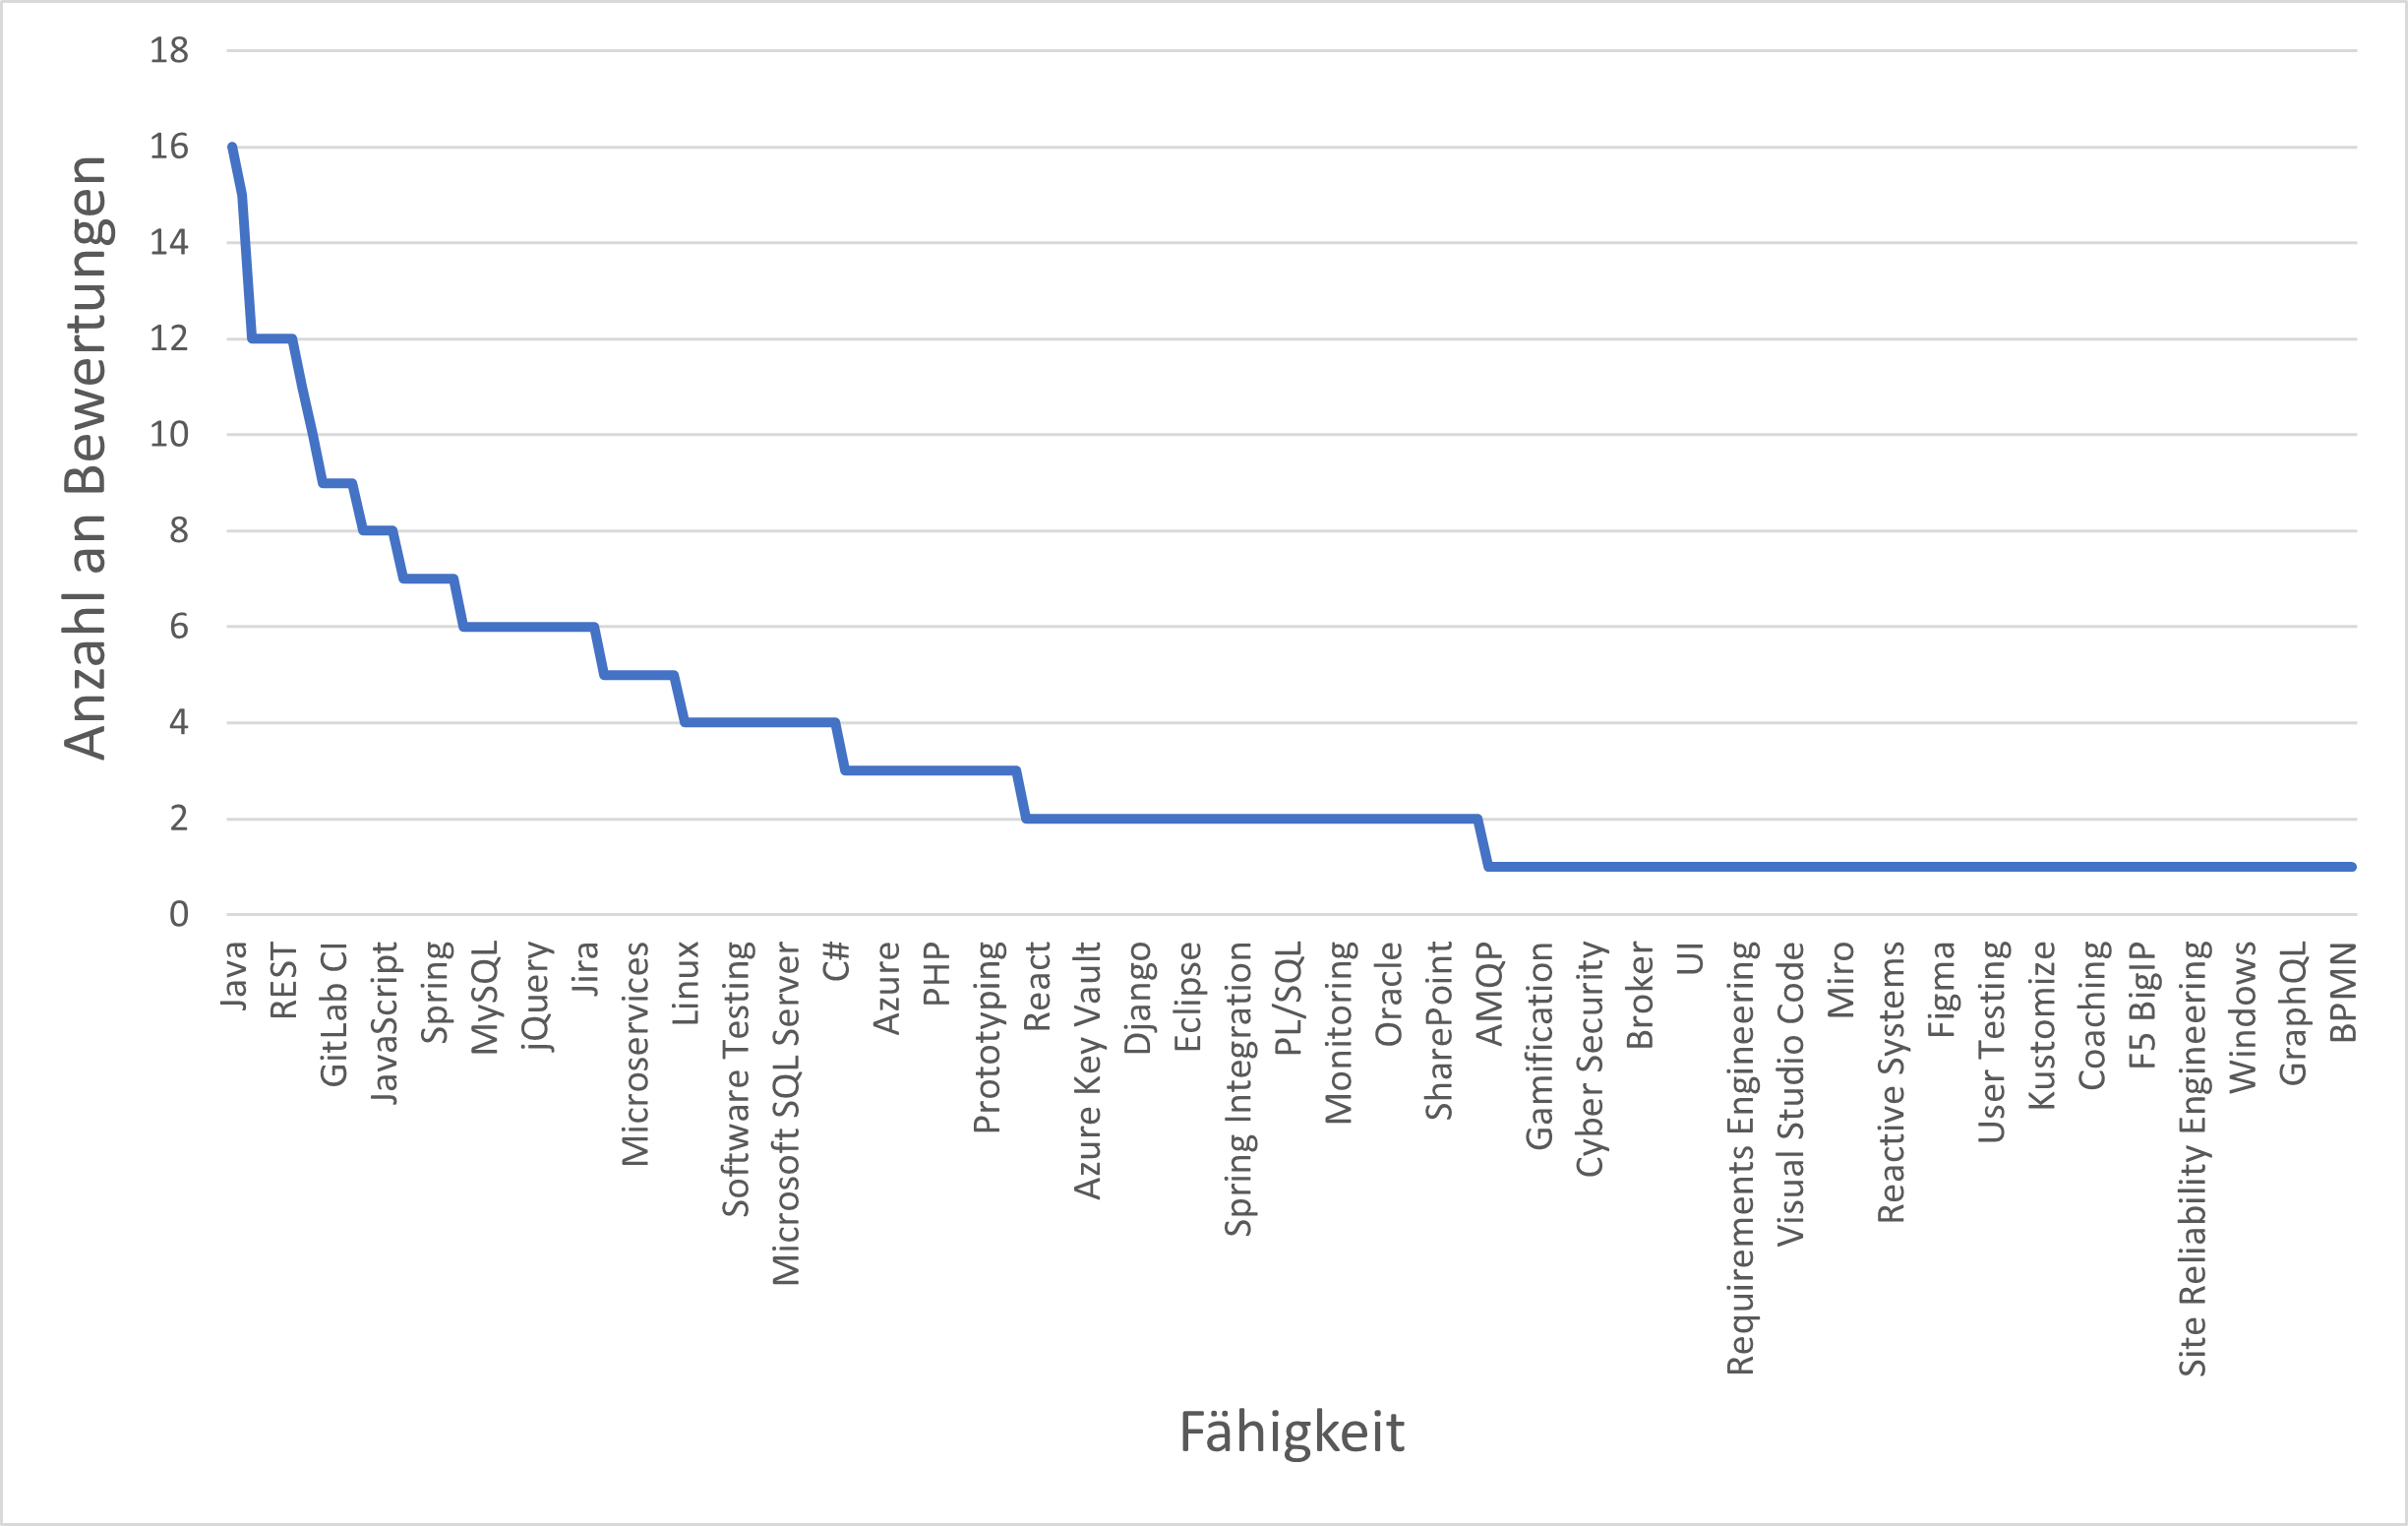
\includegraphics[width=1\textwidth]{gfx/long-tail-intranet.png}
	\caption{Langer (Ratten-)Schwanz bei den Fähigkeitsbewertungen im EXXETA-Intranet}
	\label{fig:ergebnisse:analyse:abb1}
\end{figure}

In Abbildung \ref{fig:ergebnisse:analyse:abb1} ist bezüglich des langen (Ratten-)Schwanzes festzustellen, dass neun bzw. etwa 4.3 Prozent aller Fähigkeiten über zehn oder mehr Bewertungen verfügen. Dagegen haben 151 bzw. etwa 71.2 Prozent aller Kompetenzen drei oder weniger Beurteilungen.

In den vorliegenden Daten des Intranets ist darüber hinaus zu beobachten, dass vier bzw. etwa 17.4 Prozent der Mitarbeiter keine einzige Fähigkeit bewertet haben. Diese Angestellten sind seit Einführung des Kompetenz-Bewertungssystems durchgehend in einem Projekt tätig und daher von ihrer Führungskraft noch nicht zur Pflege ihrer Fähigkeiten aufgefordert worden.

\section{Präferenzen der Mitarbeiter aus der Umfrage}
\label{ch:ergebnisse:analyse2}
Bei der Umfrage zu den Präferenzen haben die Mitarbeiter insgesamt 1408 Bewertungen abgegeben, welche sich auf 370 einzelne Kompetenzen verteilen. Dies entspricht knapp über 61 abgegebenen Wünschen pro Mitarbeiter. Git ist mit 18 Beurteilungen die meist präferierte Fähigkeit. Wie in Abbildung \ref{fig:ergebnisse:analyse:abb2} zu erkennen, deutet sich auch hinsichtlich der Wünsche ein langer (Ratten-)Schwanz an, wenn die Fähigkeiten nach Anzahl an Beurteilungen sortiert dargestellt werden.
 
\begin{figure}[h]
	\centering
	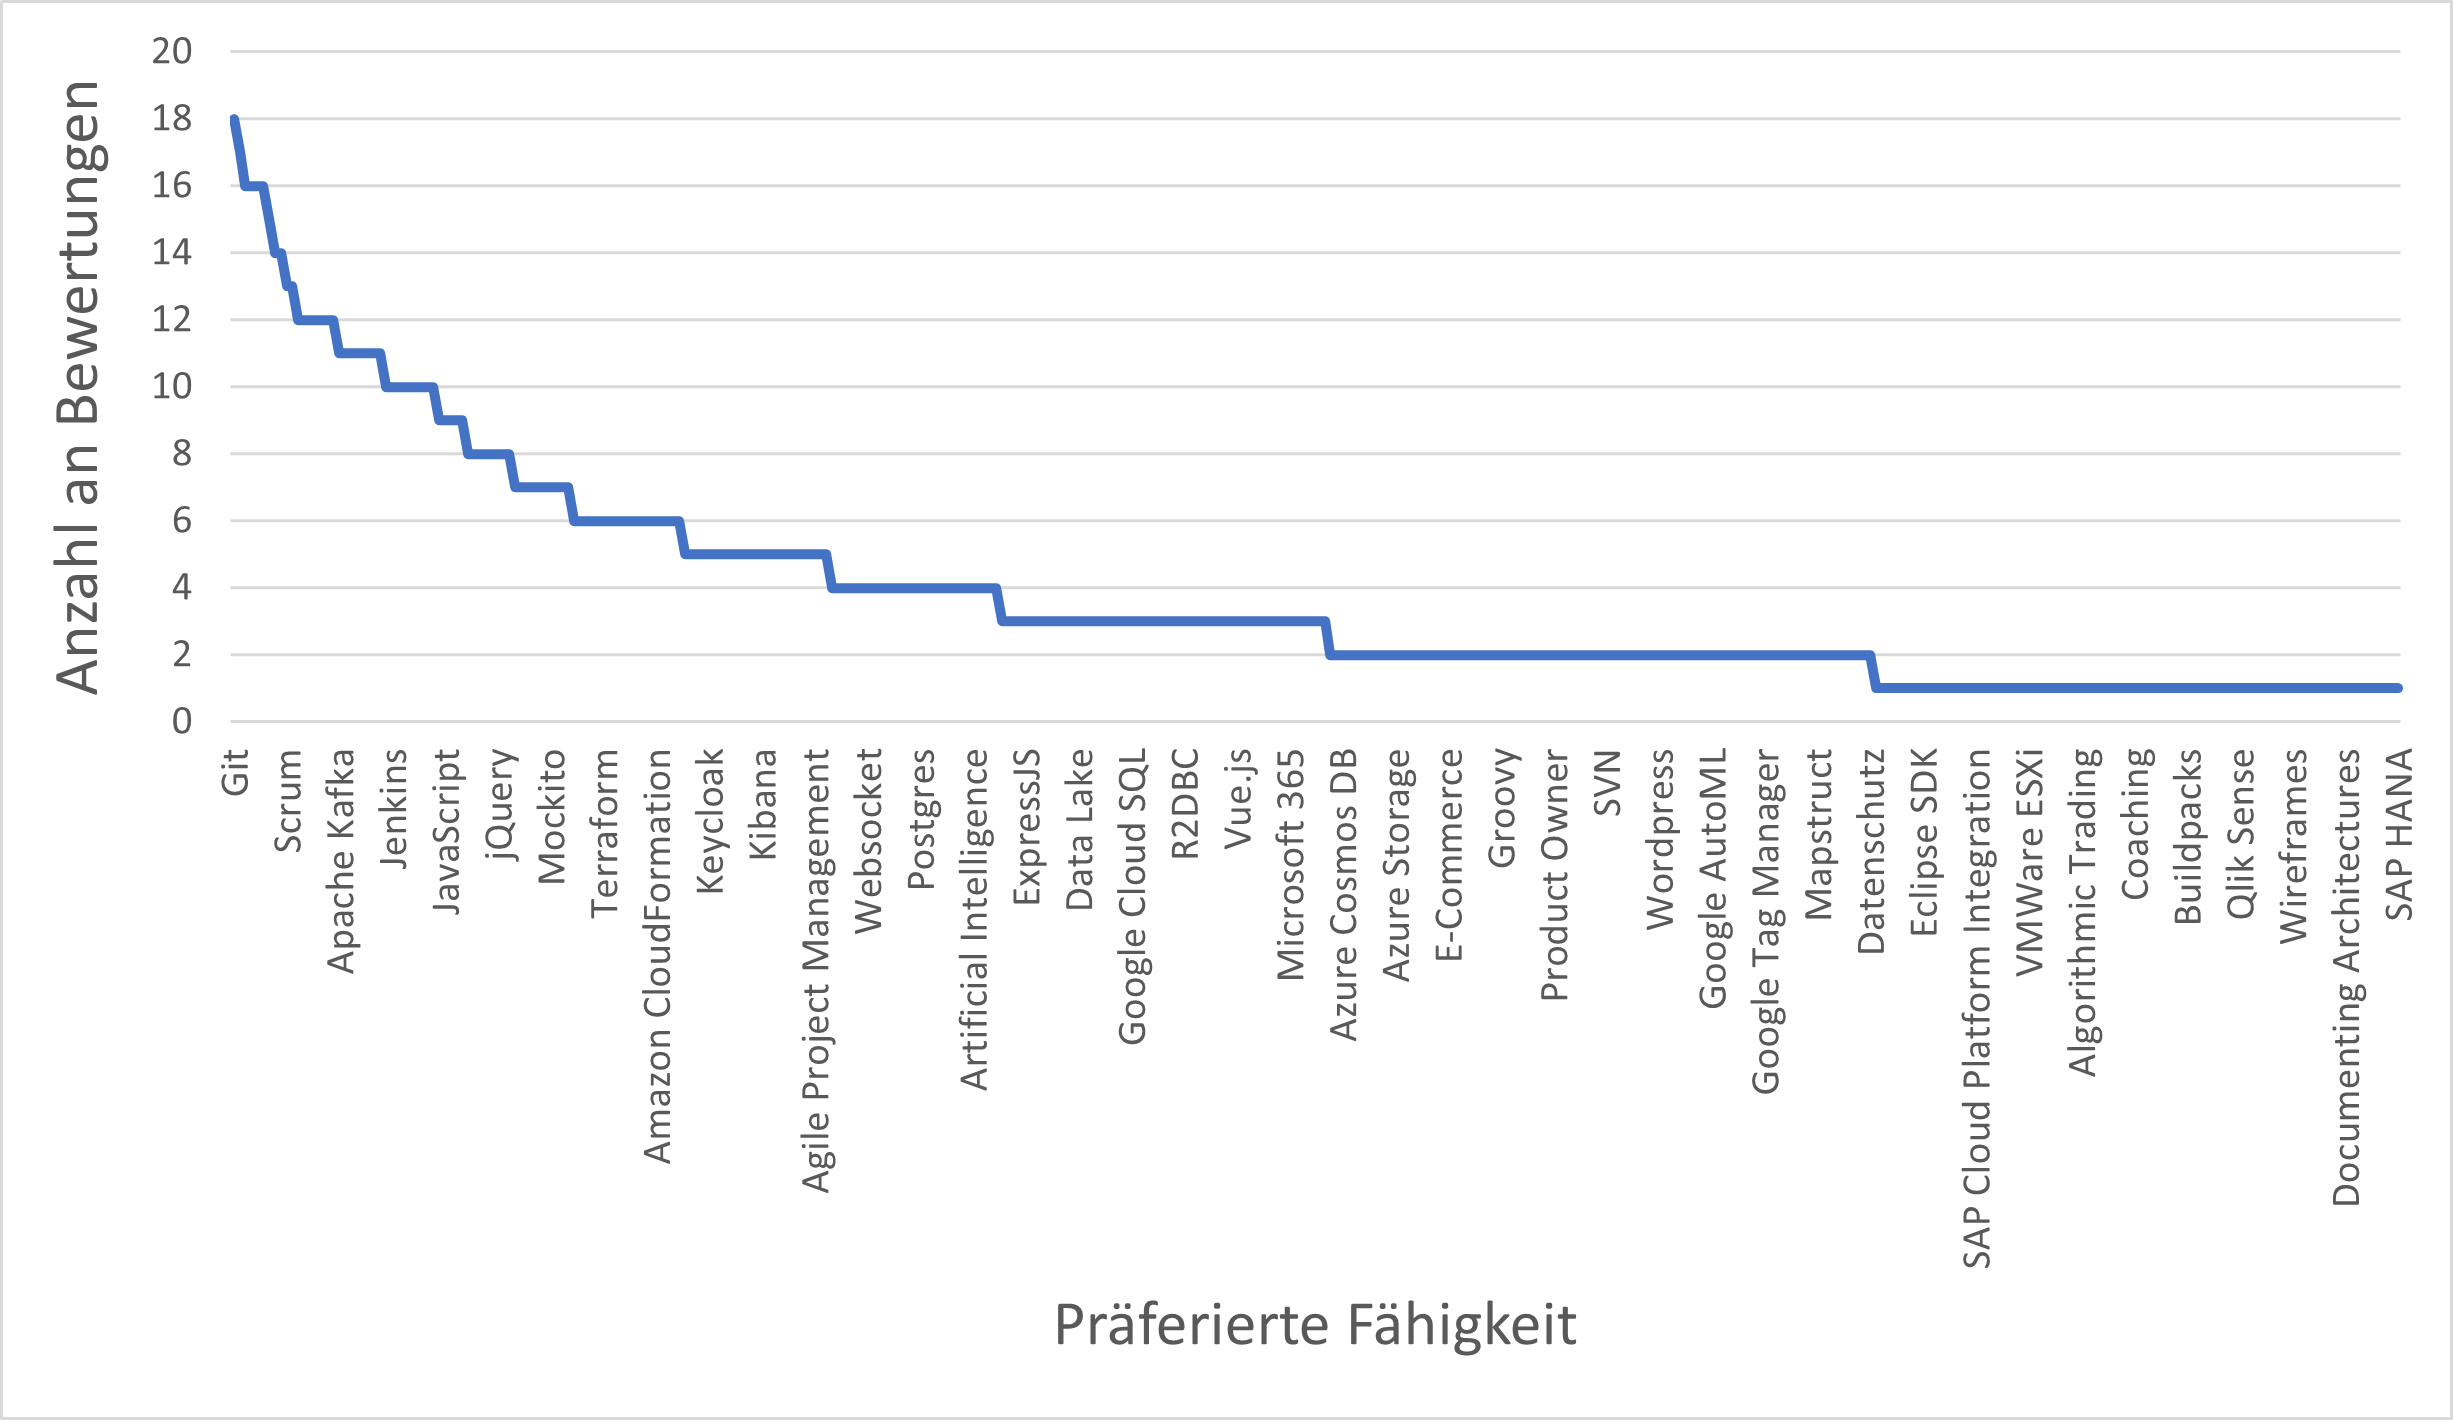
\includegraphics[width=1\textwidth]{gfx/long-tail-praeferenzen.png}
	\caption{Langer (Ratten-)Schwanz bei den präferierten Fähigkeiten der Mitarbeiter}
	\label{fig:ergebnisse:analyse:abb2}
\end{figure}

Zu Abbildung \ref{fig:ergebnisse:analyse:abb2} ist festzustellen, dass 18 bzw. etwa 4.9 Prozent aller Fähigkeiten von zwölf oder mehr Mitarbeitern präferiert werden. Dem gegenüber stehen 268 bzw. etwa 72.4 Prozent aller Kompetenzen, welche vier oder weniger Angestellte als Wunsch angegeben haben. Bei der Umfrage gab es keinen Mitarbeiter, welcher keine einzige Fähigkeit als Präferenz ausgewählte.

\section{Gemeinsame Betrachtung beherrschter und präferierter Fähigkeiten}
\label{ch:ergebnisse:analyse3}
Bei der gemeinsamen Betrachtung von Kompetenzen und Wünschen ist auf Mitarbeiterebene festzustellen, dass ein durchschnittlicher Angestellter etwa 74.7 Fähigkeiten beherrscht und/oder präferiert. Abbildung \ref{fig:ergebnisse:analyse:abb3} zeigt, wie viele dieser Kompetenzen der durchschnittliche Mitarbeiter beherrscht und wie viele er davon präferiert.

\begin{figure}[h]
	\centering
	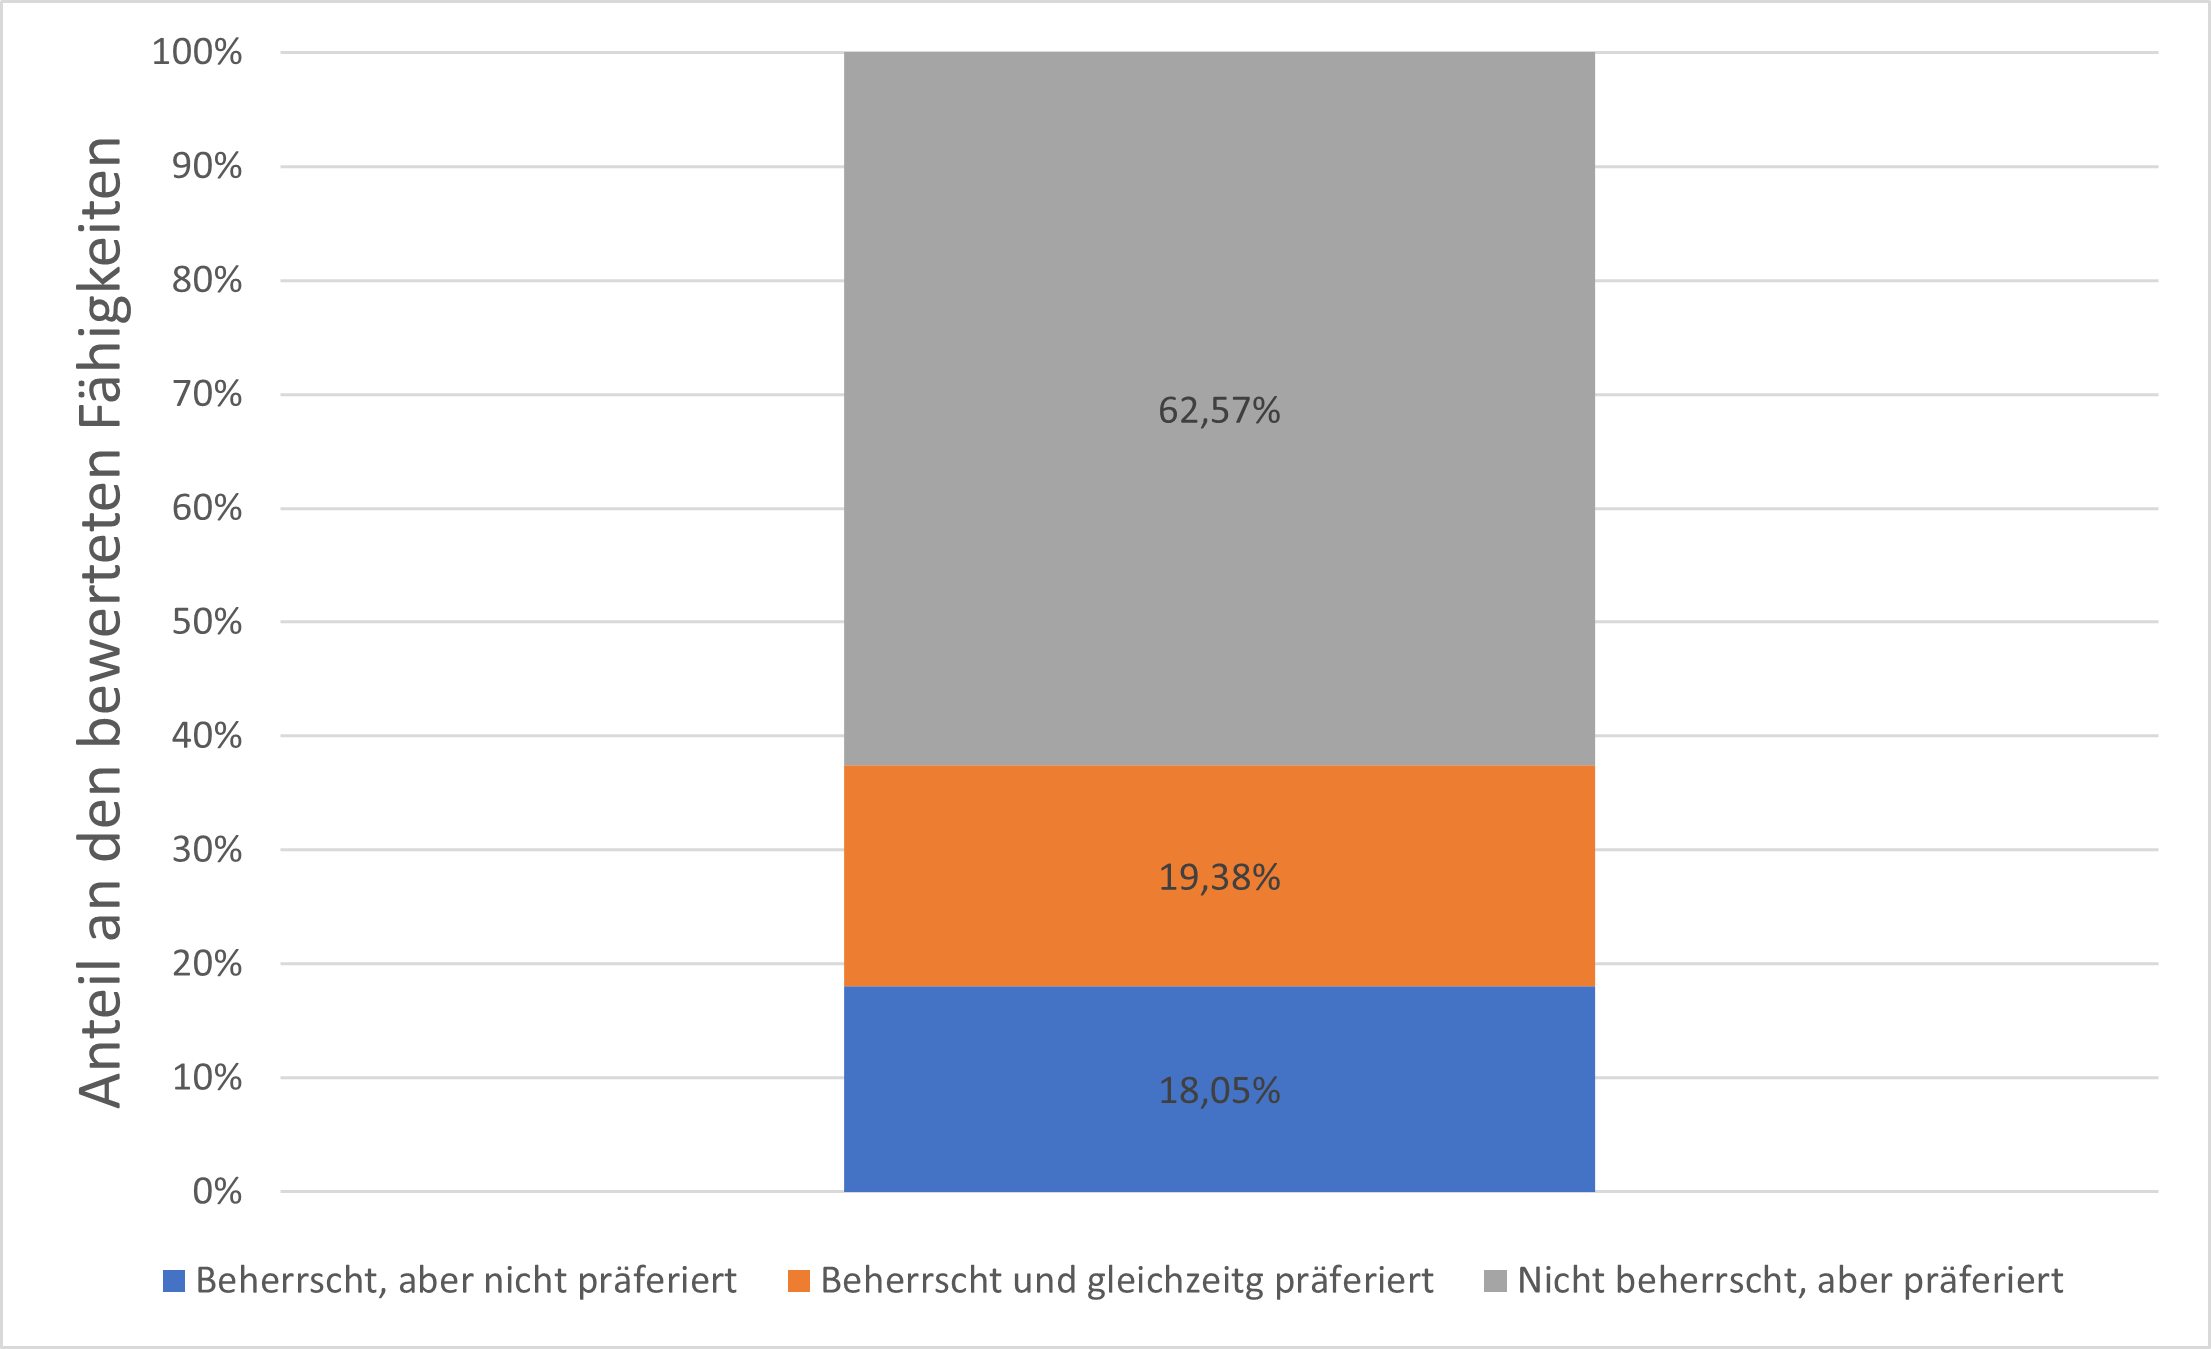
\includegraphics[width=0.9\textwidth]{gfx/auswertung-anteil-an-faehigkeiten.png}
	\caption{Anteil beherrschter und präferierter Fähigkeiten bei einem durchschnittlichen Mitarbeiter}
	\label{fig:ergebnisse:analyse:abb3}
\end{figure}

In Abbildung \ref{fig:ergebnisse:analyse:abb3} ist zu erkennen, dass ein durchschnittlicher Angestellter etwa 28 bzw. ca. 37.4 Prozent seiner insgesamt beurteilten Kompetenzen gleichzeitig beherrscht. Von diesen Fähigkeiten präferiert er jedoch nur ca. 14.5, also knapp über die Hälfte. Demgegenüber stehen ca. 46.7 bzw. etwa 62.6 Prozent an Fähigkeiten, welche der Angestellte zwar präferiert, aber noch nicht beherrscht.

Bei Betrachtung der beherrschten Fähigkeiten ist festzustellen, dass kaum Unterschiede zwischen präferierten und nicht gewünschten Kompetenzen ausgemacht werden können. So verfügt die durchschnittliche beherrschte, aber nicht gewünschte Fähigkeit (blaue Farbe in Abbildung \ref{fig:ergebnisse:analyse:abb3}) über eine Bewertung von 2.9 im Intranet. Die durchschnittliche vorhandene und gleichzeitig präferierte Kompetenz (orangene Farbe in Abbildung \ref{fig:ergebnisse:analyse:abb3}) verfügt über eine Bewertung von 3.1. Wie in Abbildung \ref{fig:ergebnisse:analyse:abb4} zu erkennen, sind auch bei Betrachtung der Fähigkeiten auf ihren jeweiligen Kompetenzniveaus kaum Differenzen auszumachen.

\begin{figure}[h]
	\centering
	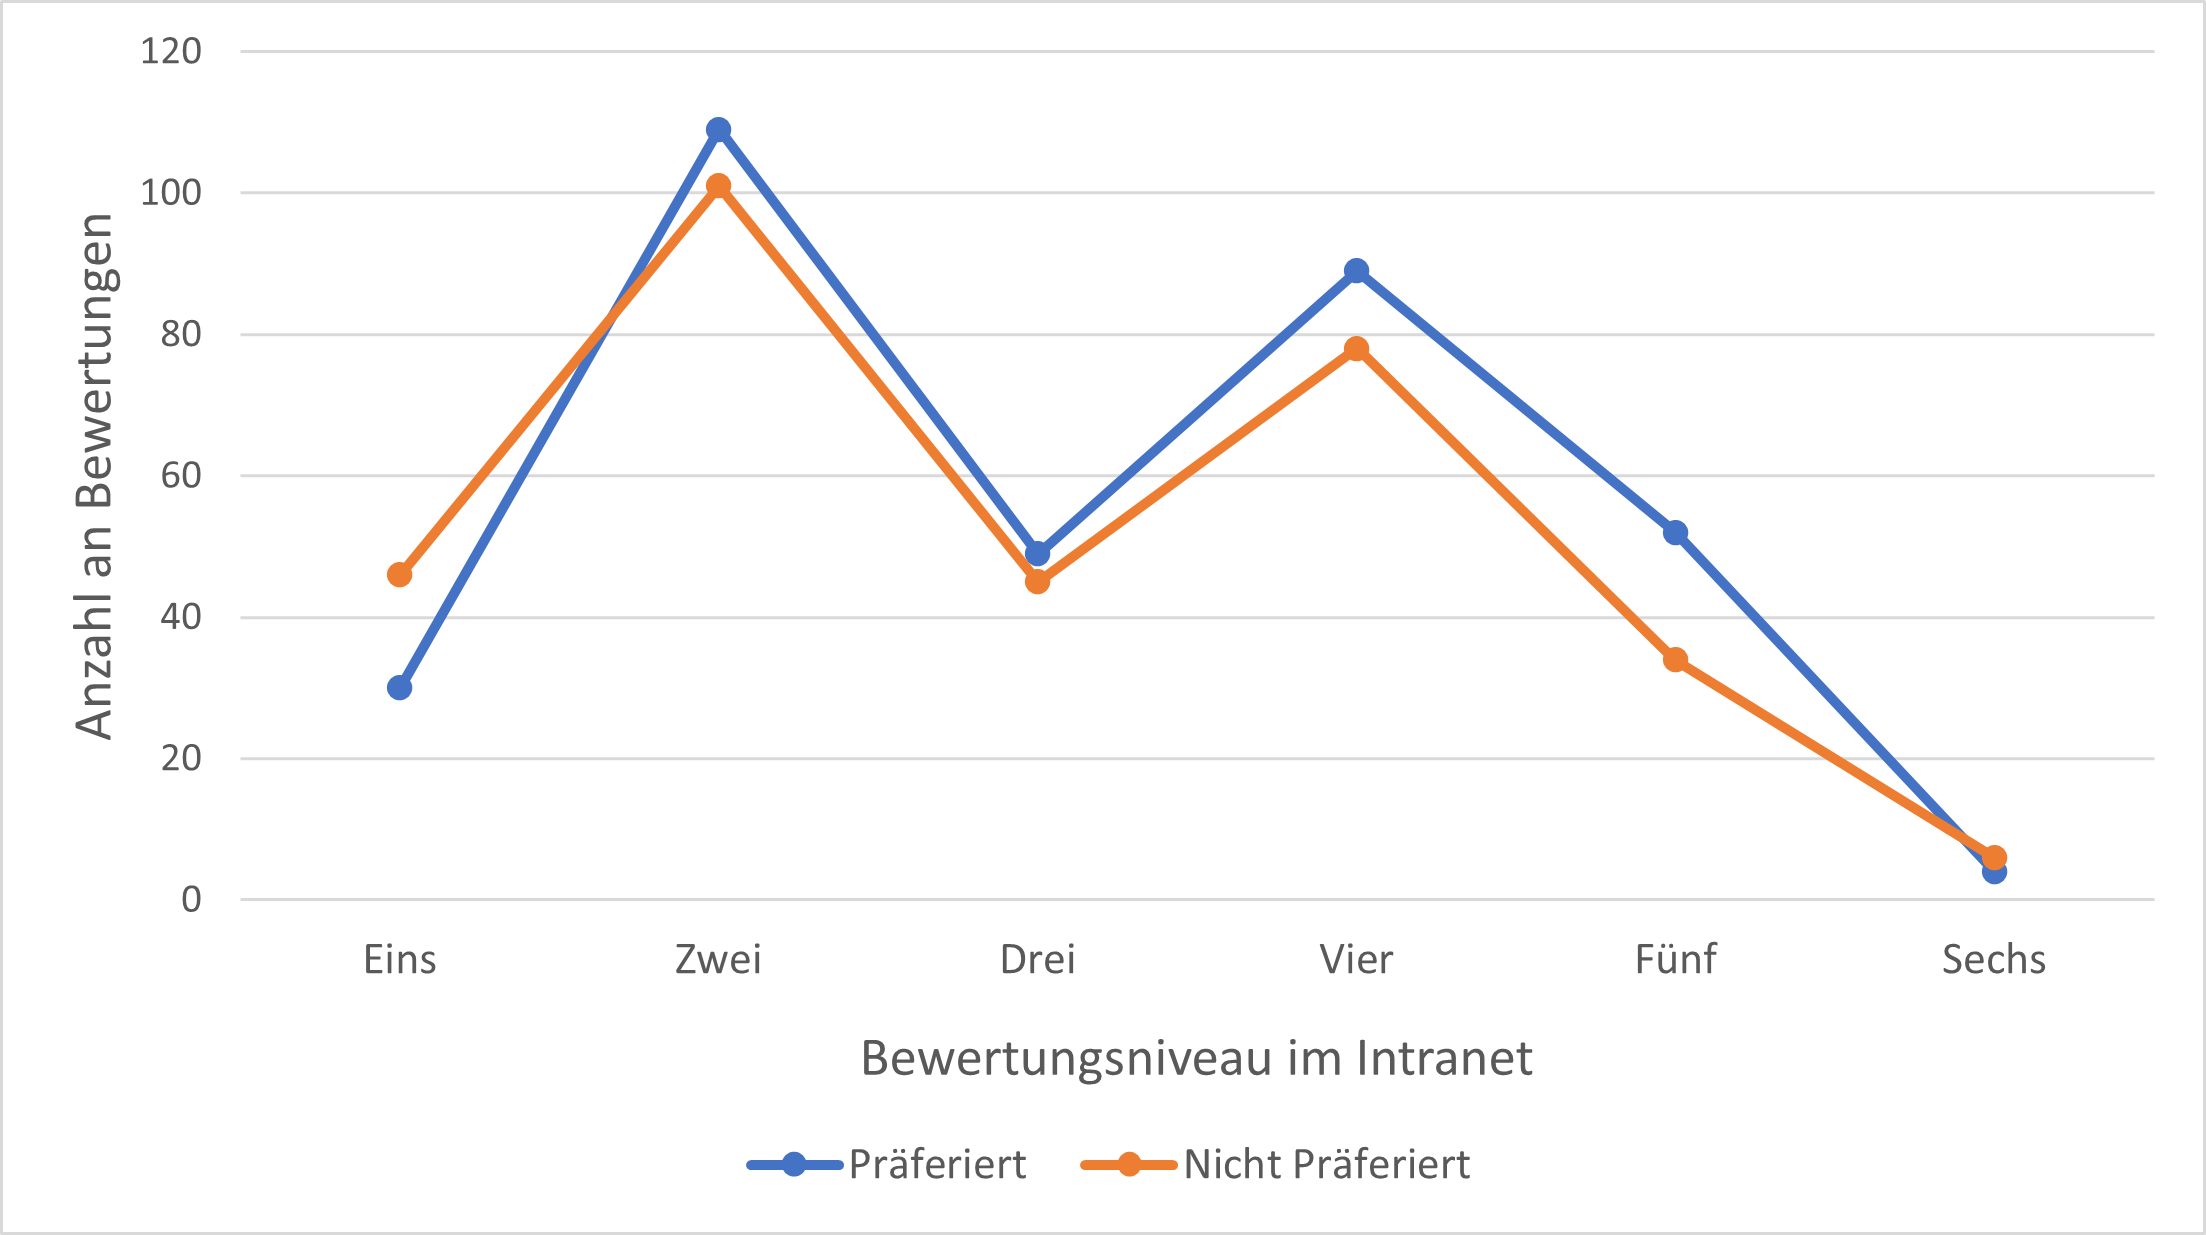
\includegraphics[width=0.8\textwidth]{gfx/bewertungen-je-bewertungsniveau.png}
	\caption{Anzahl beherrschter und präferierter Fähigkeiten je Bewertungsniveau}
	\label{fig:ergebnisse:analyse:abb4}
\end{figure}

Bei Analyse der präferierten Fähigkeiten (graue Farbe in Abbildung \ref{fig:ergebnisse:analyse:abb3}) ist zu beobachten, dass es sich bei den meist gewünschten Kompetenzen hauptsächlich um moderne Produkte aus dem Web- und Cloud-Umfeld handelt. So zählen neben Git und Java beispielsweise Kotlin, Kubernetes, Docker, Spring Boot und AWS zu den meist präferierten Fähigkeiten.

\section{Analyse der Beispielprojektpositionen}
\label{ch:ergebnisse:projekte}
Bei Betrachtung der in den fünf Beispielprojektpositionen aus Abbildung \ref{fig:methodik:evaluation:abb2} gesuchten Fähigkeiten ist festzustellen, dass 67 Prozent aller Mitarbeiter die durchschnittlich gesuchte 

\begin{figure}[h]
	\centering
	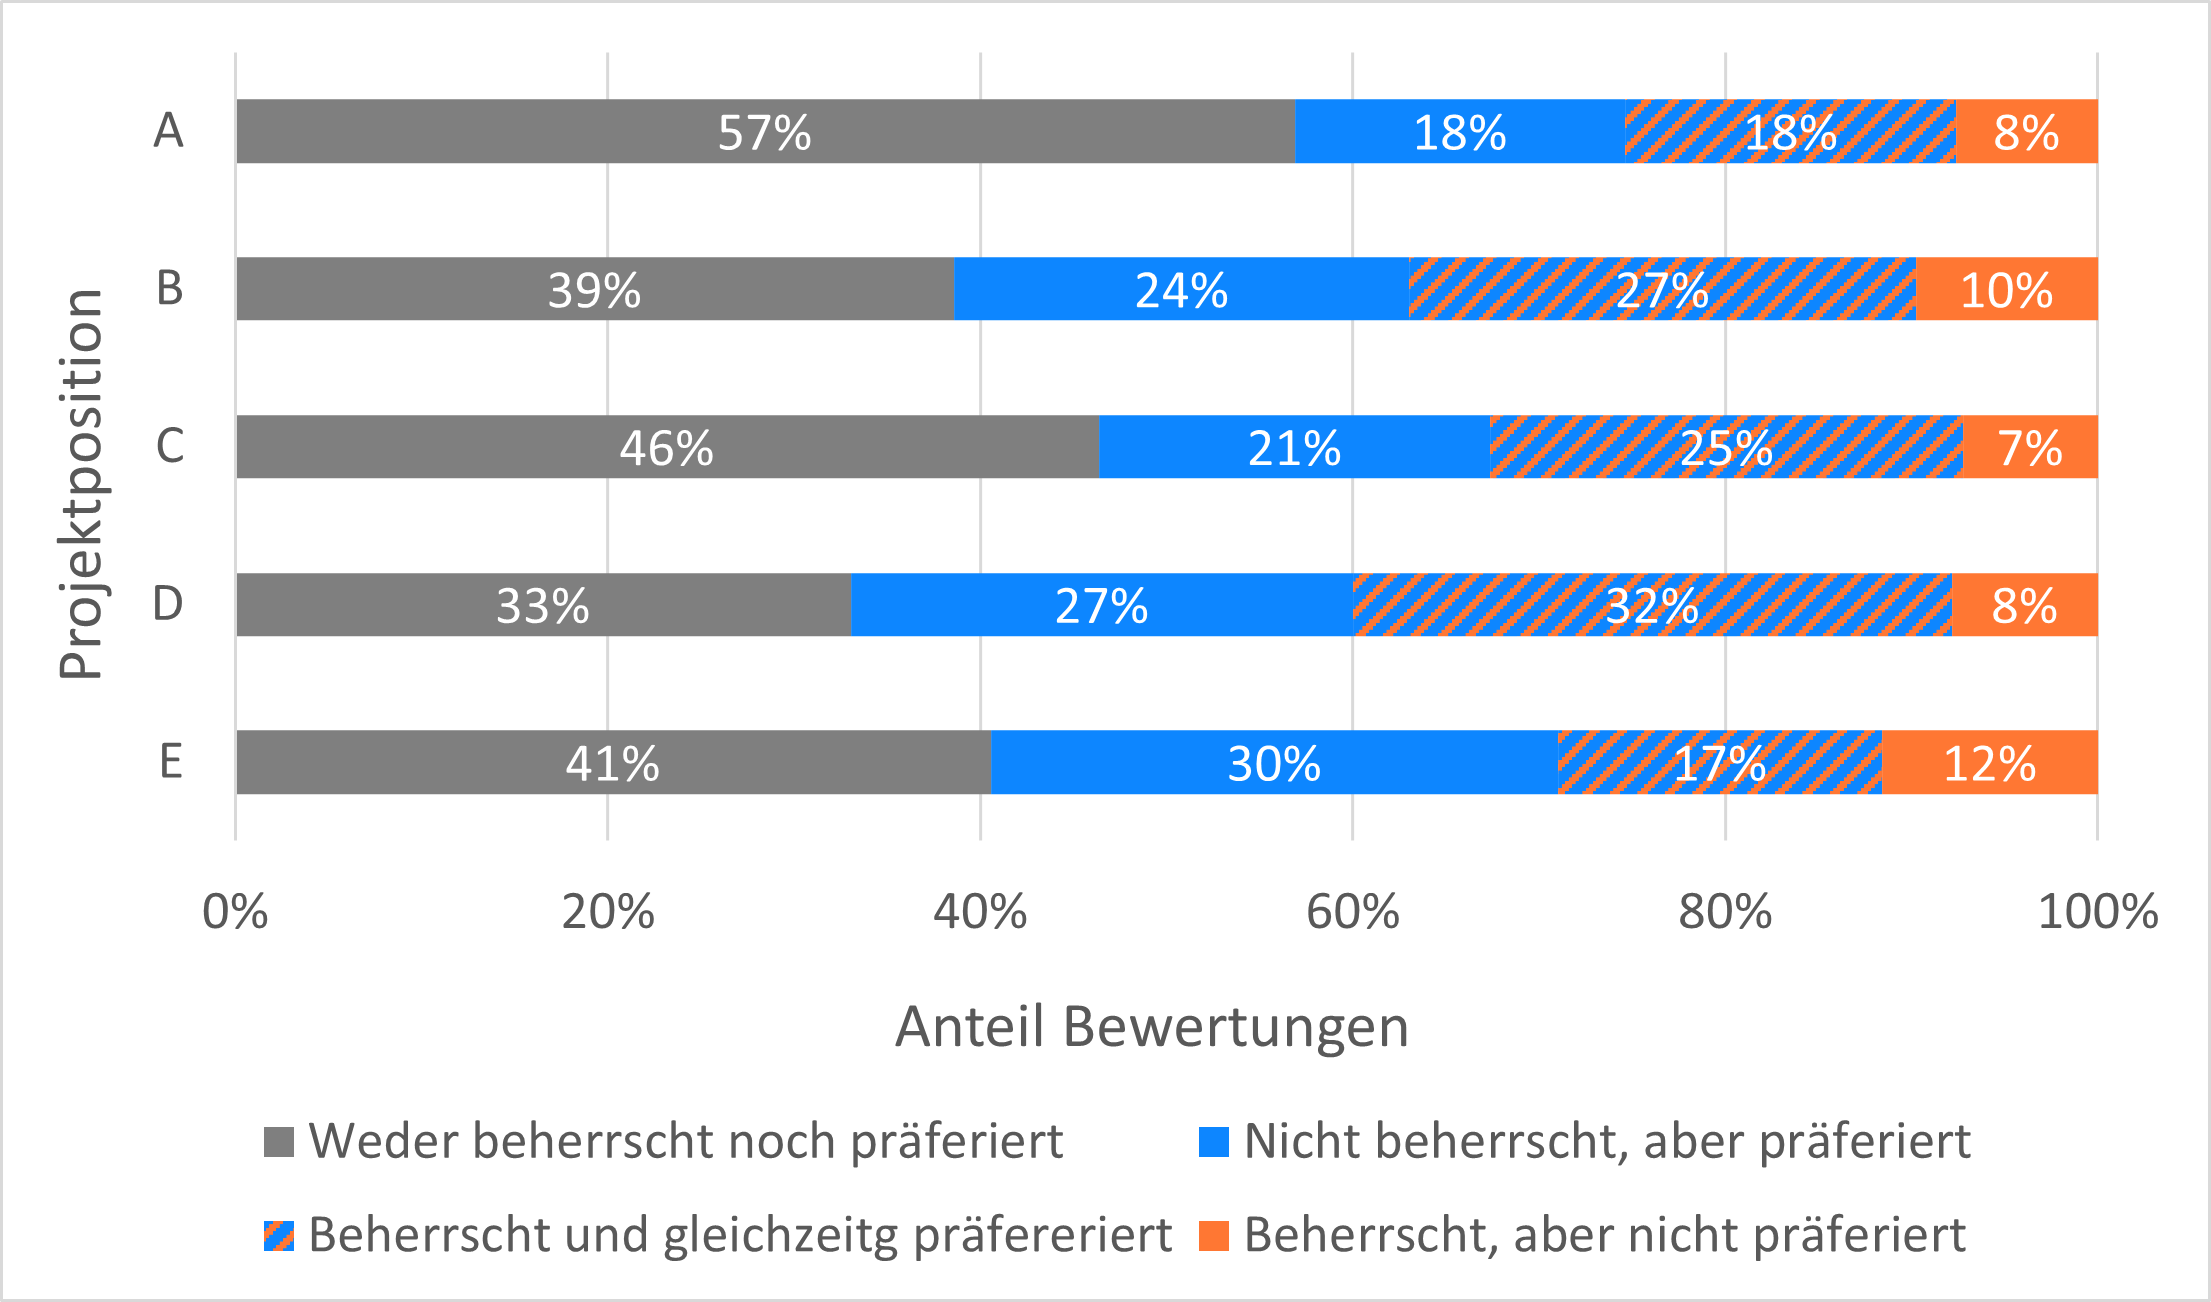
\includegraphics[width=1\textwidth]{gfx/anteil-bewertungen-je-projektposition.png}
	\caption{Anzahl beherrschter und präferierter Fähigkeiten je Bewertungsniveau TODO}
	\label{fig:ergebnisse:analyse:abb5}
\end{figure}

xxx

\begin{figure}[h]
	\centering
	
	\subfloat[Projektposition A]{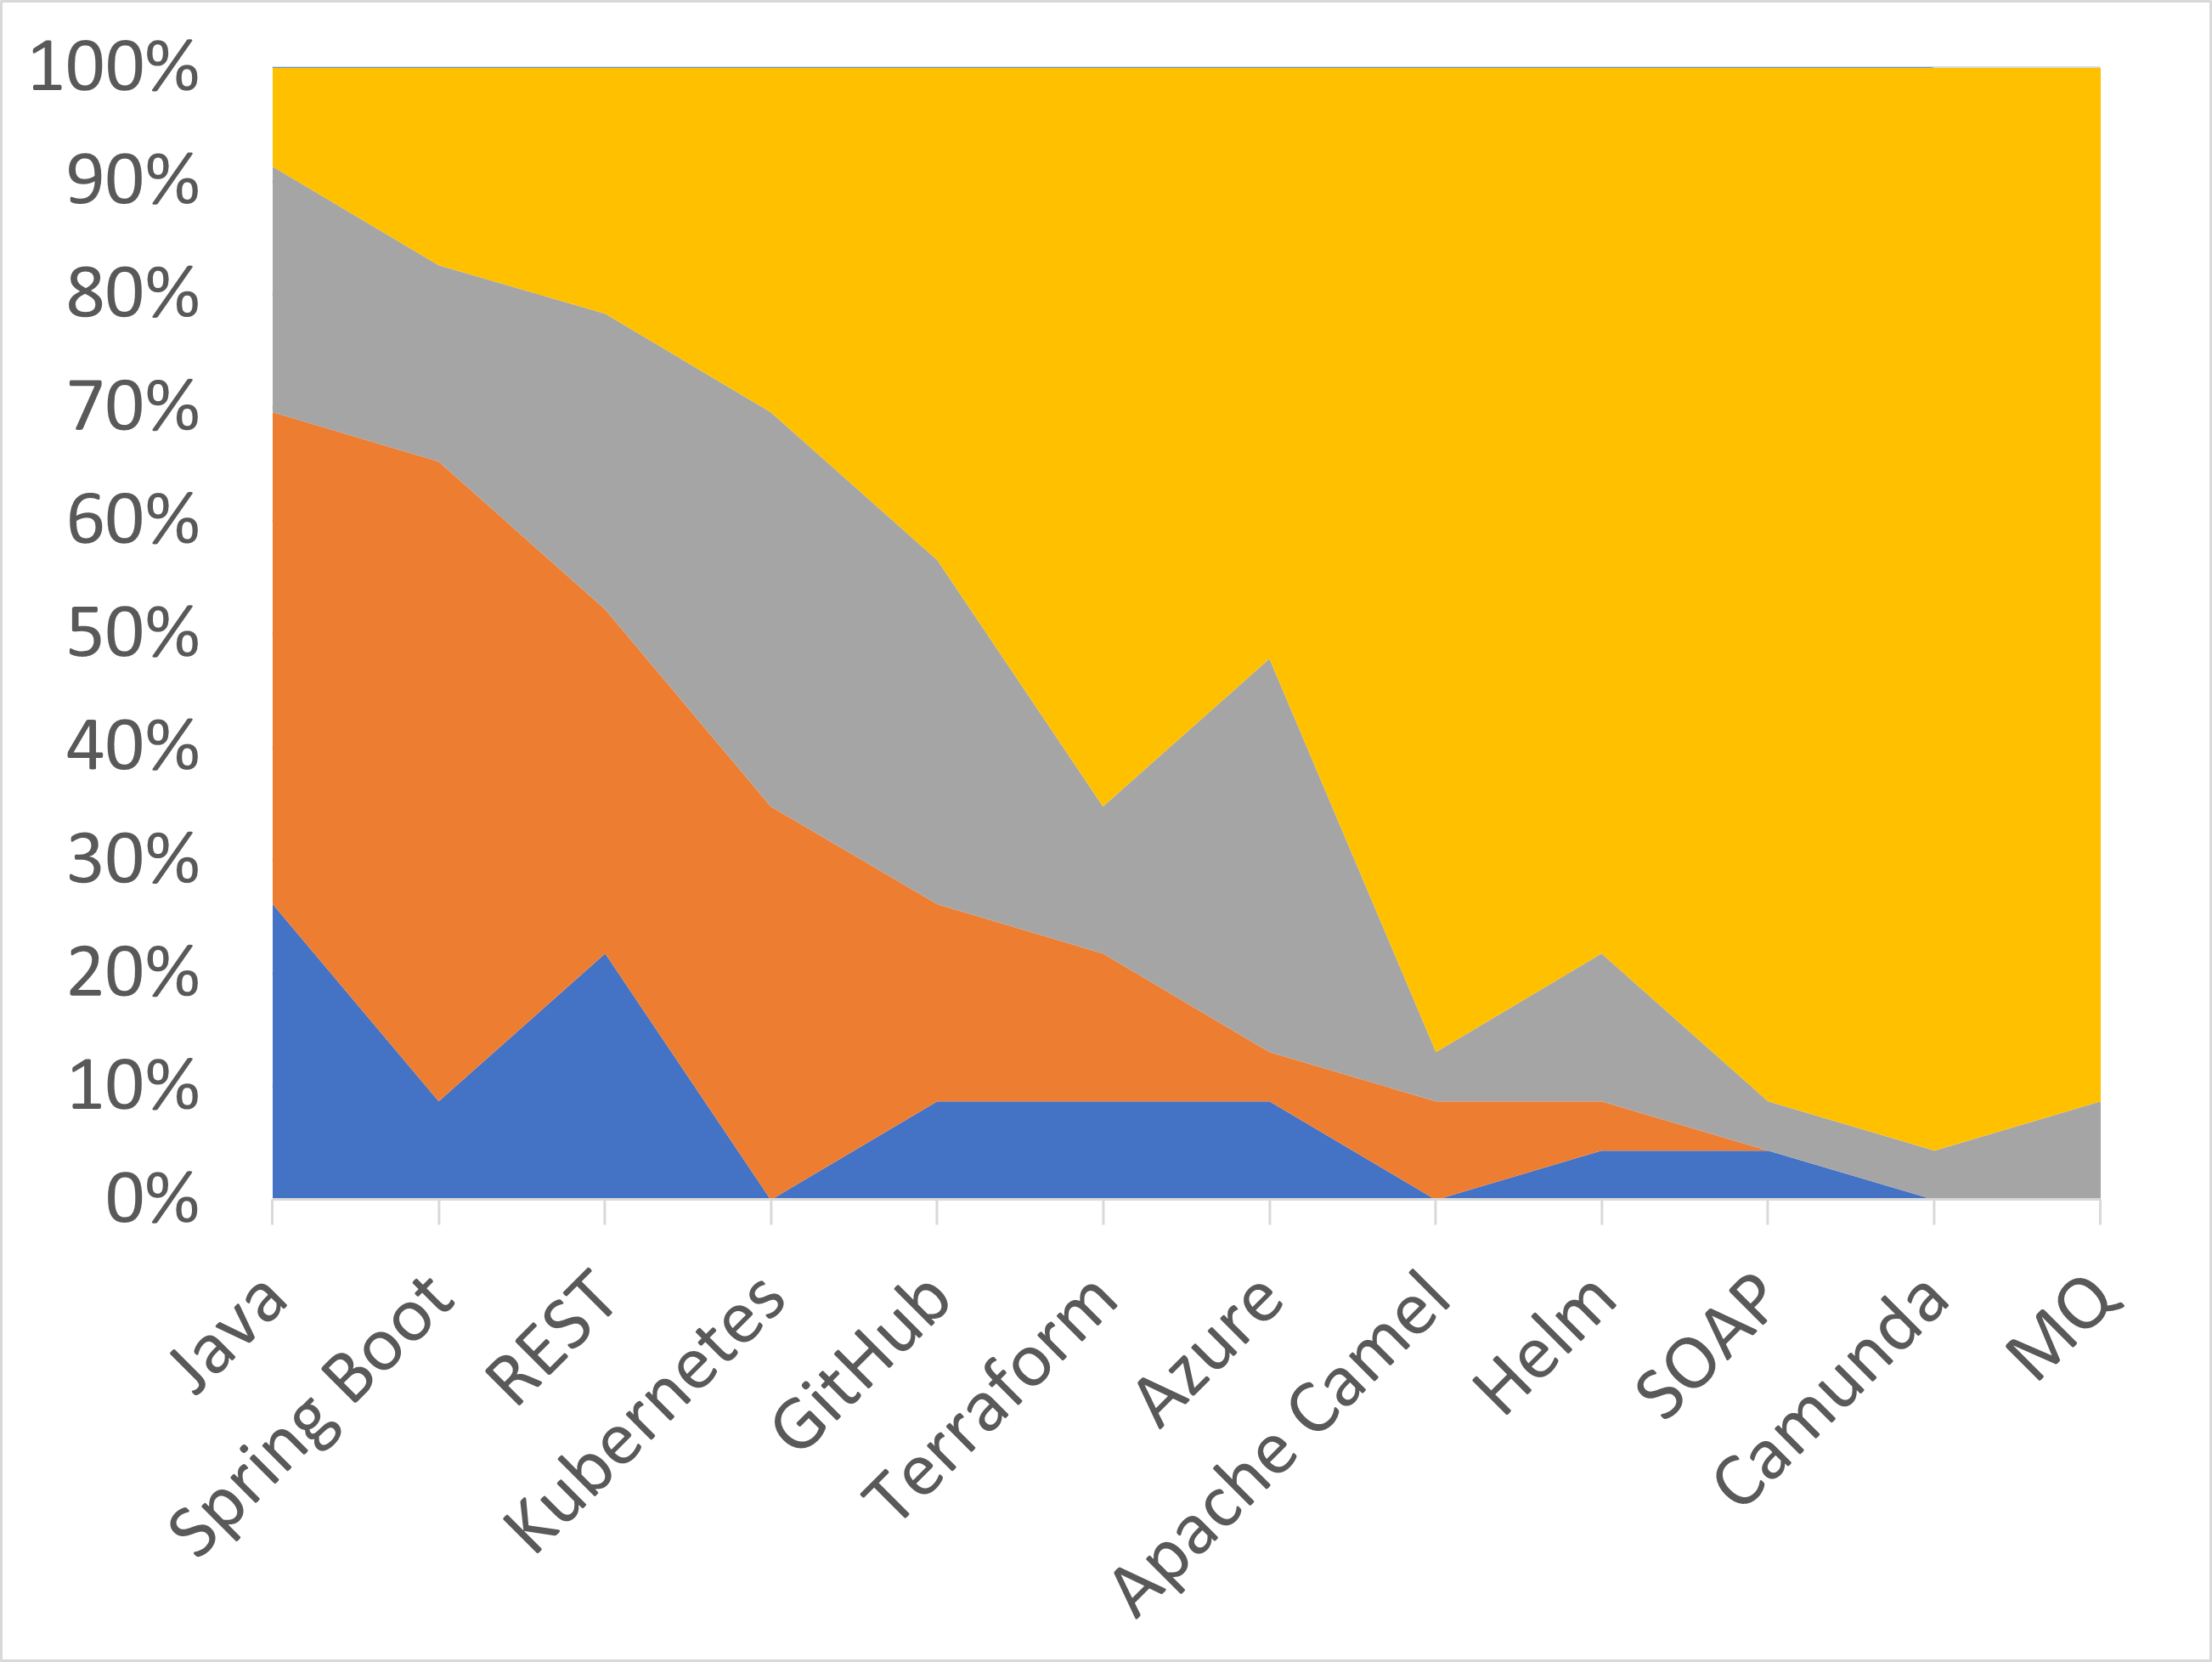
\includegraphics[width = 0.5\textwidth]{gfx/projekt-detail-a.png}}
	\subfloat[Projektposition B]{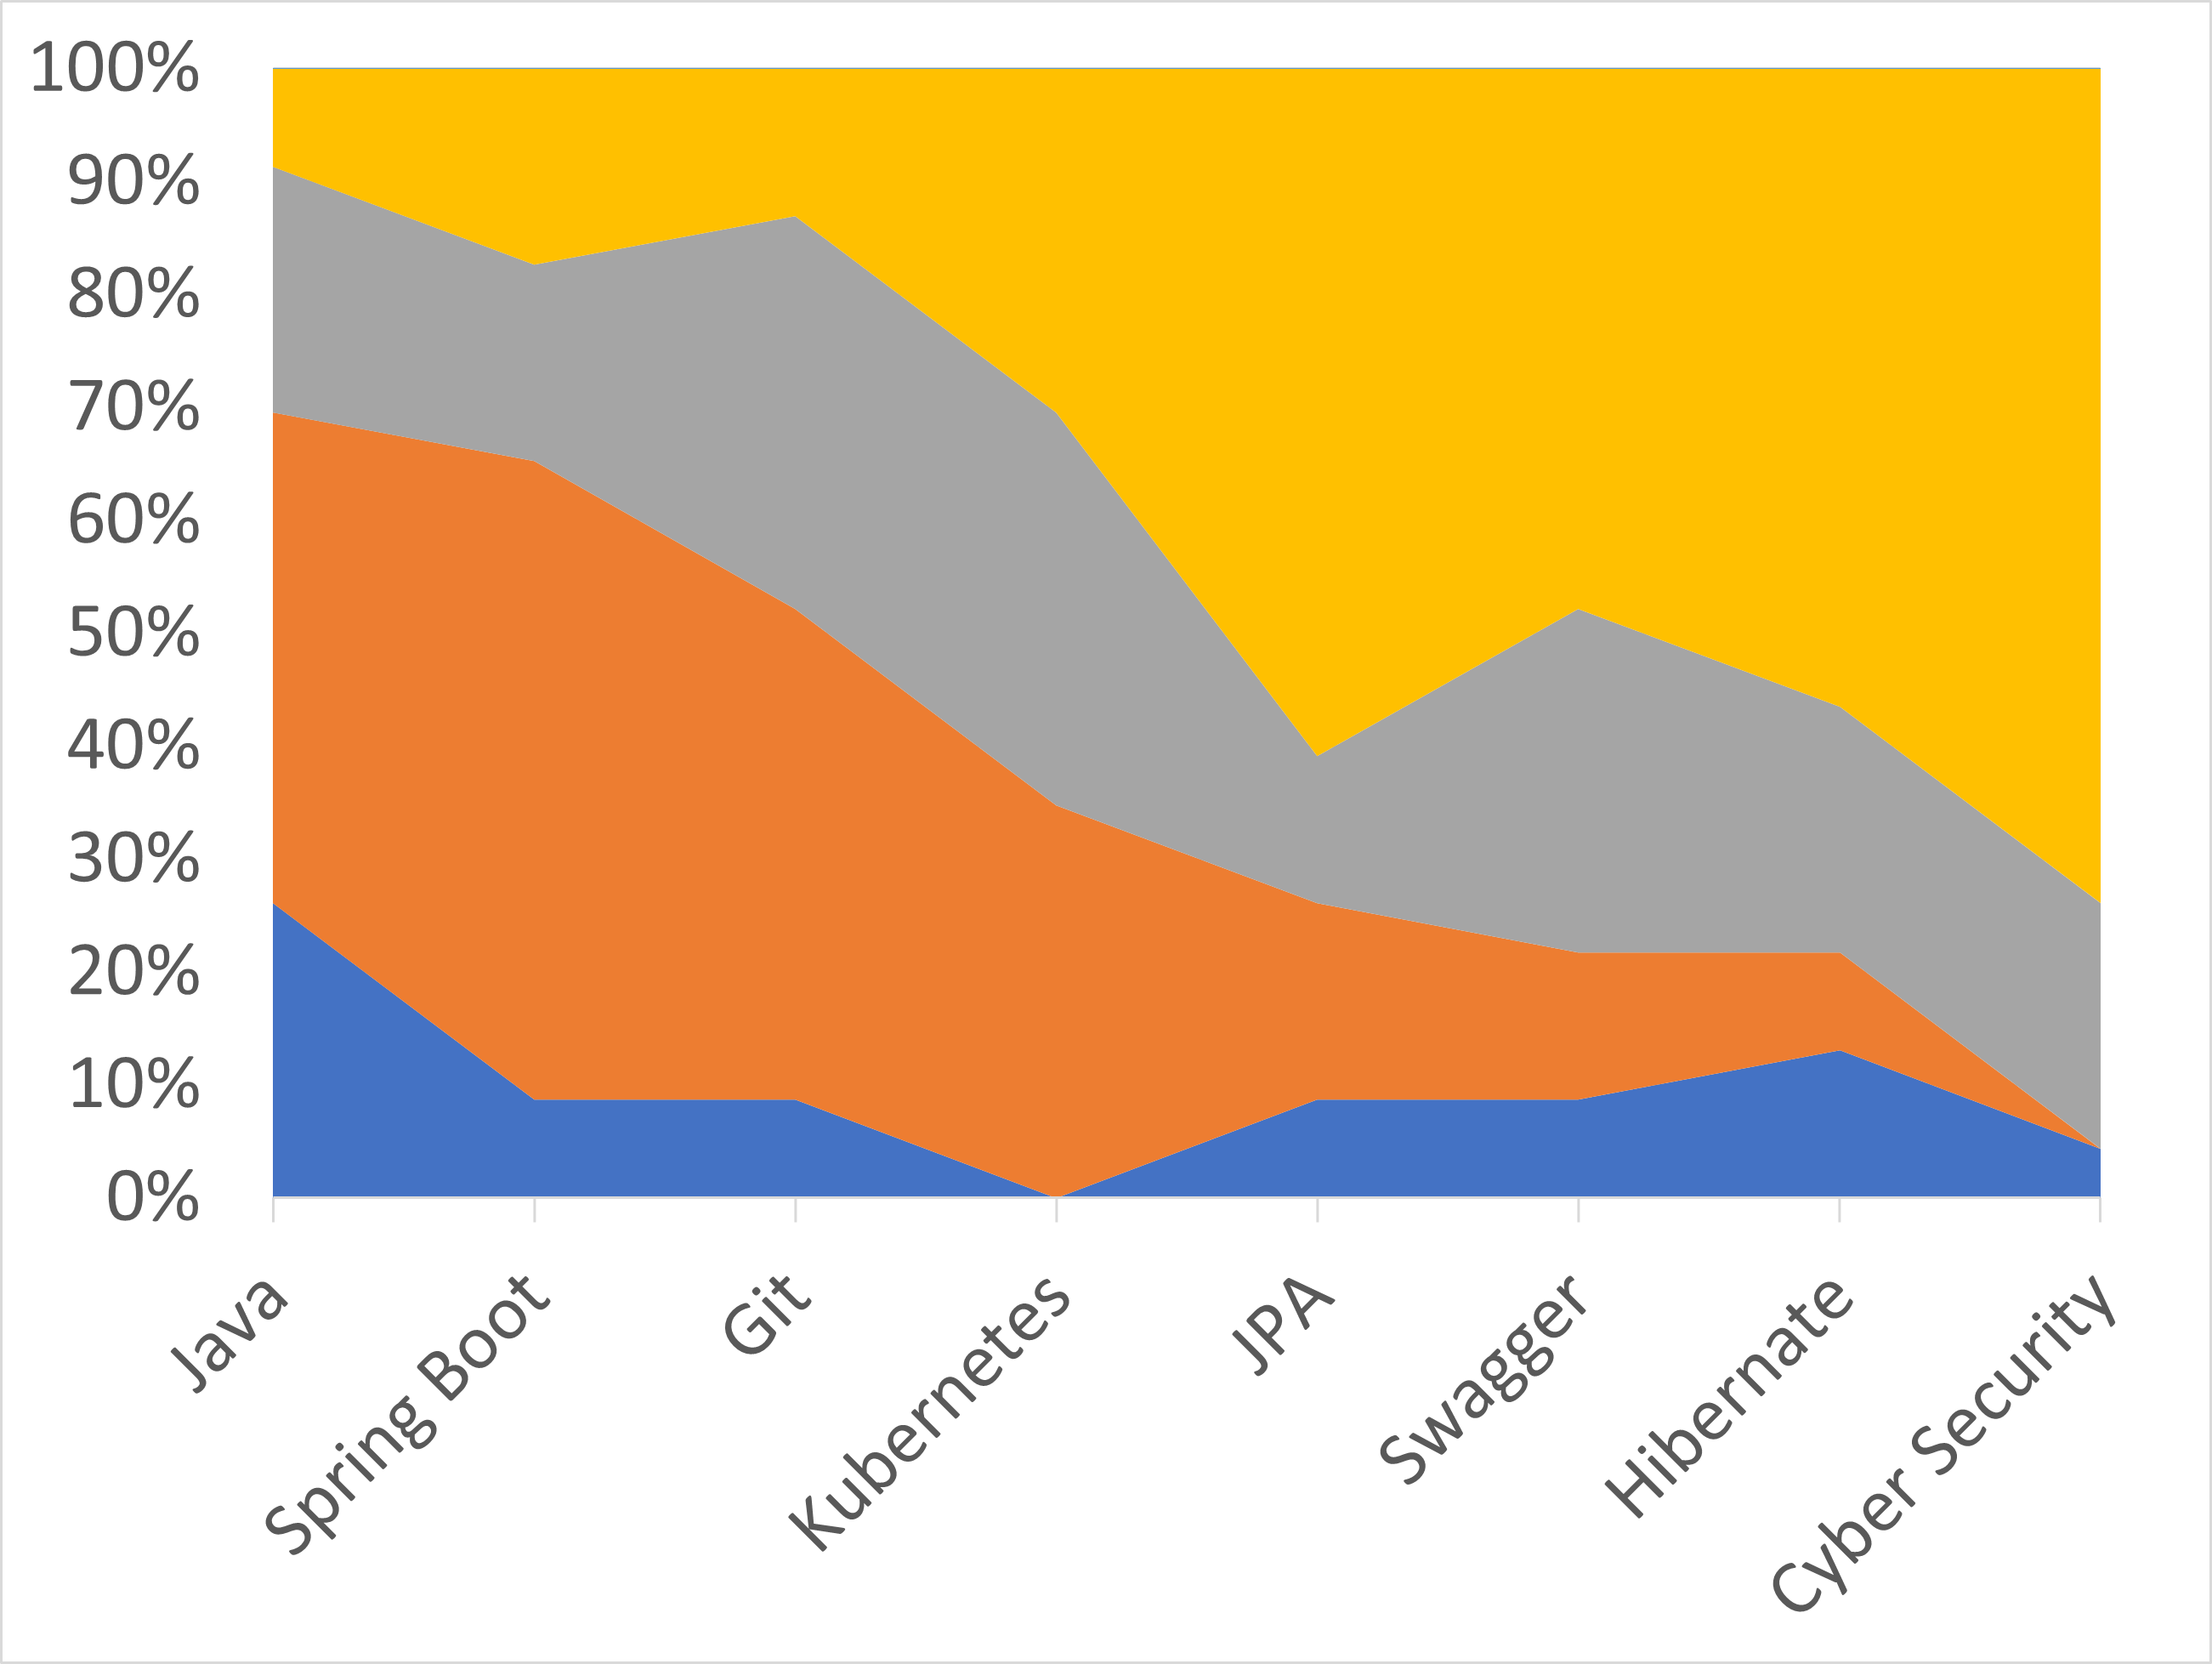
\includegraphics[width = 0.5\textwidth]{gfx/projekt-detail-b.png}}
	\newline
	\subfloat[Projektposition C]{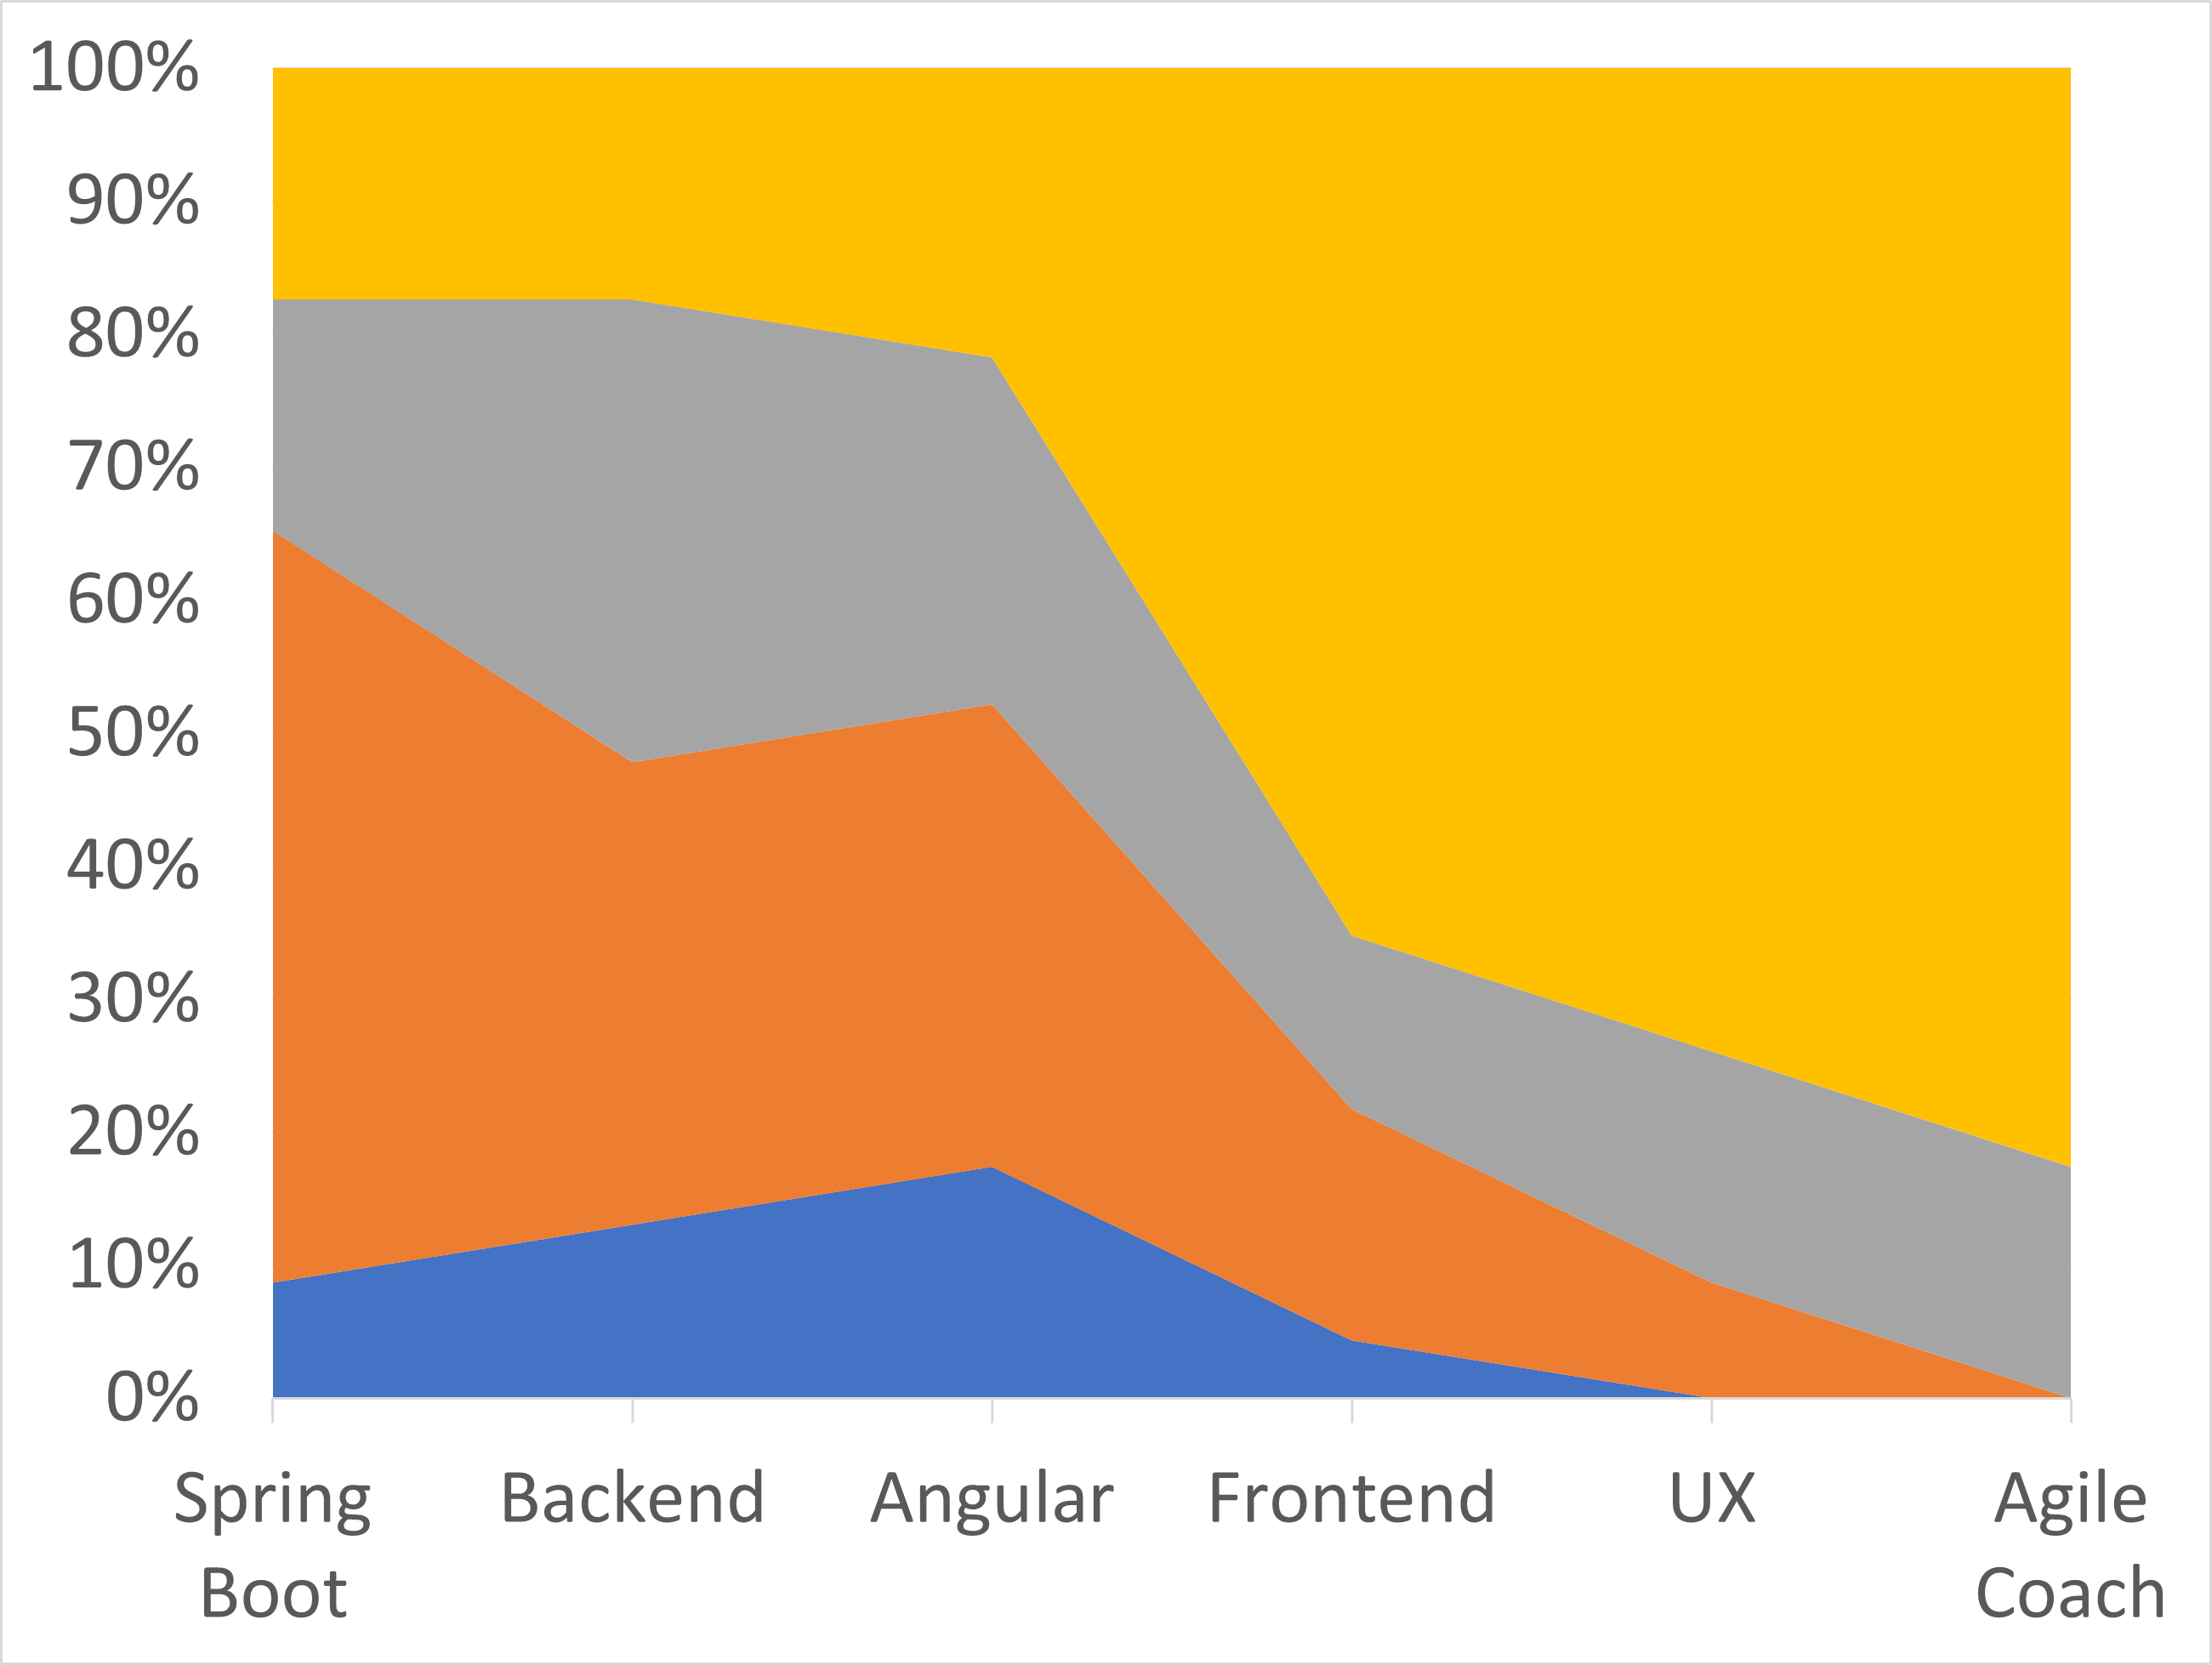
\includegraphics[width = 0.5\textwidth]{gfx/projekt-detail-c.png}}
	\subfloat[Projektposition D]{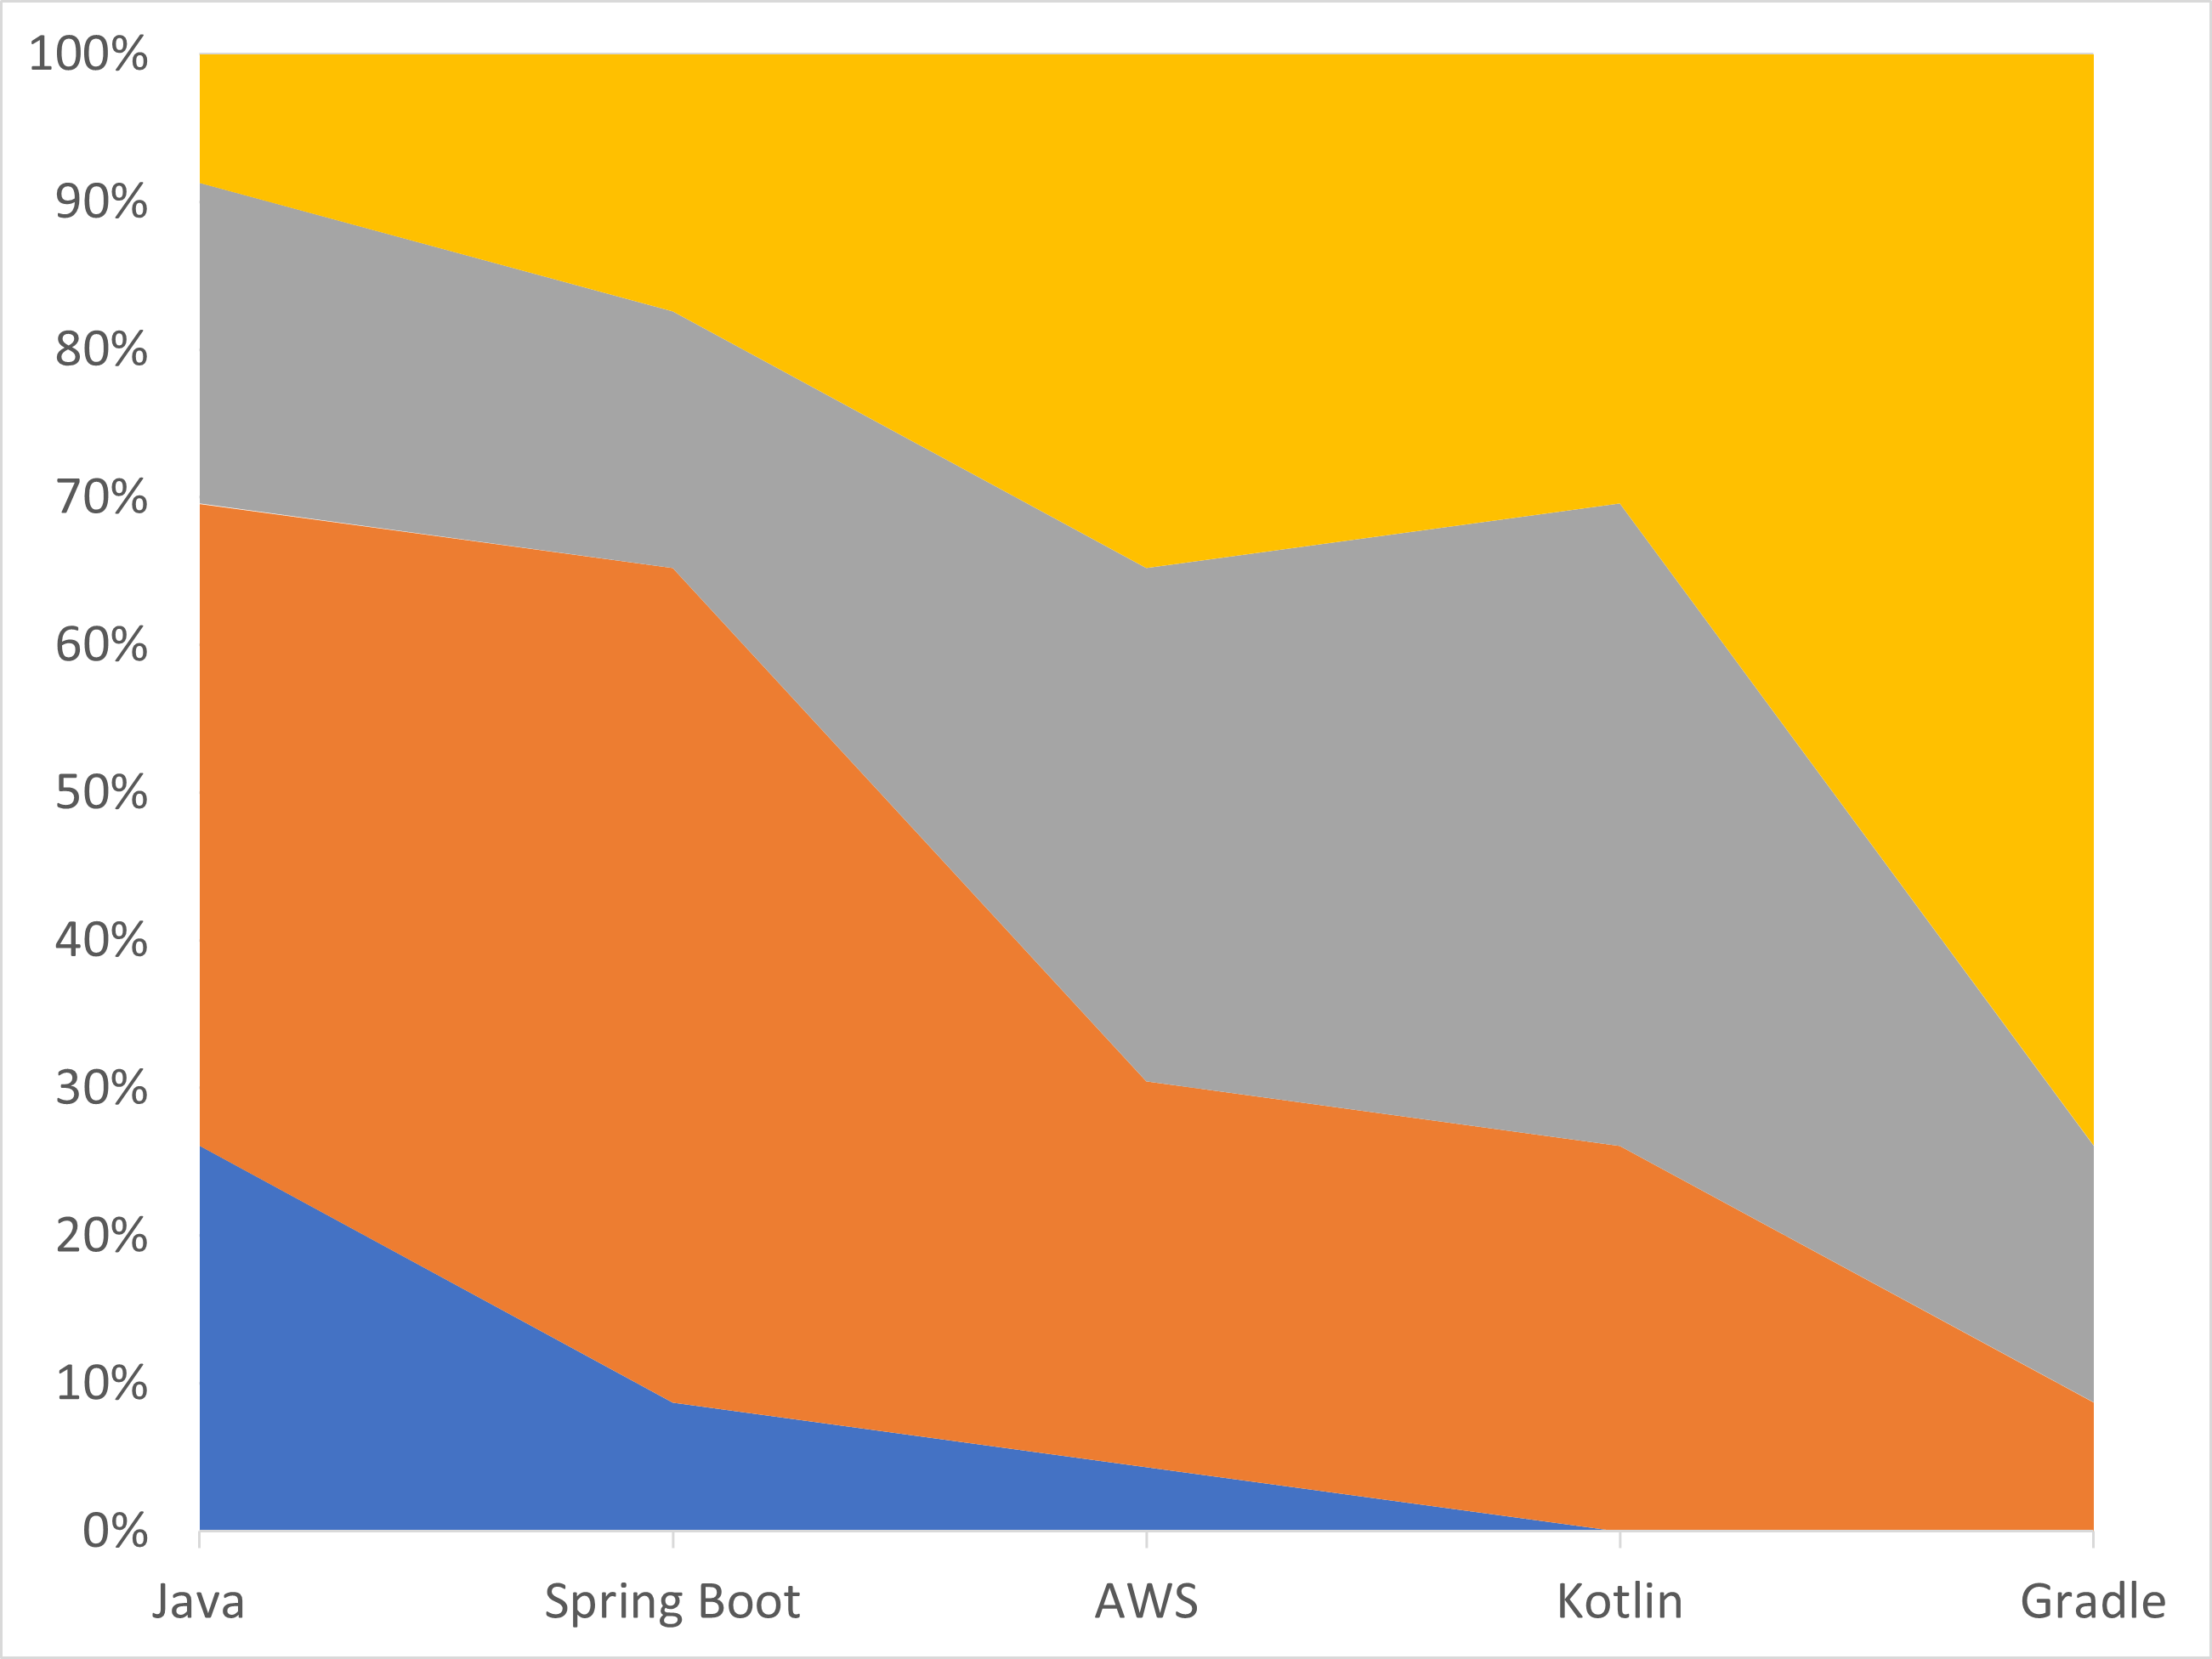
\includegraphics[width = 0.5\textwidth]{gfx/projekt-detail-d.png}}
	\newline
	\subfloat[Projektposition E]{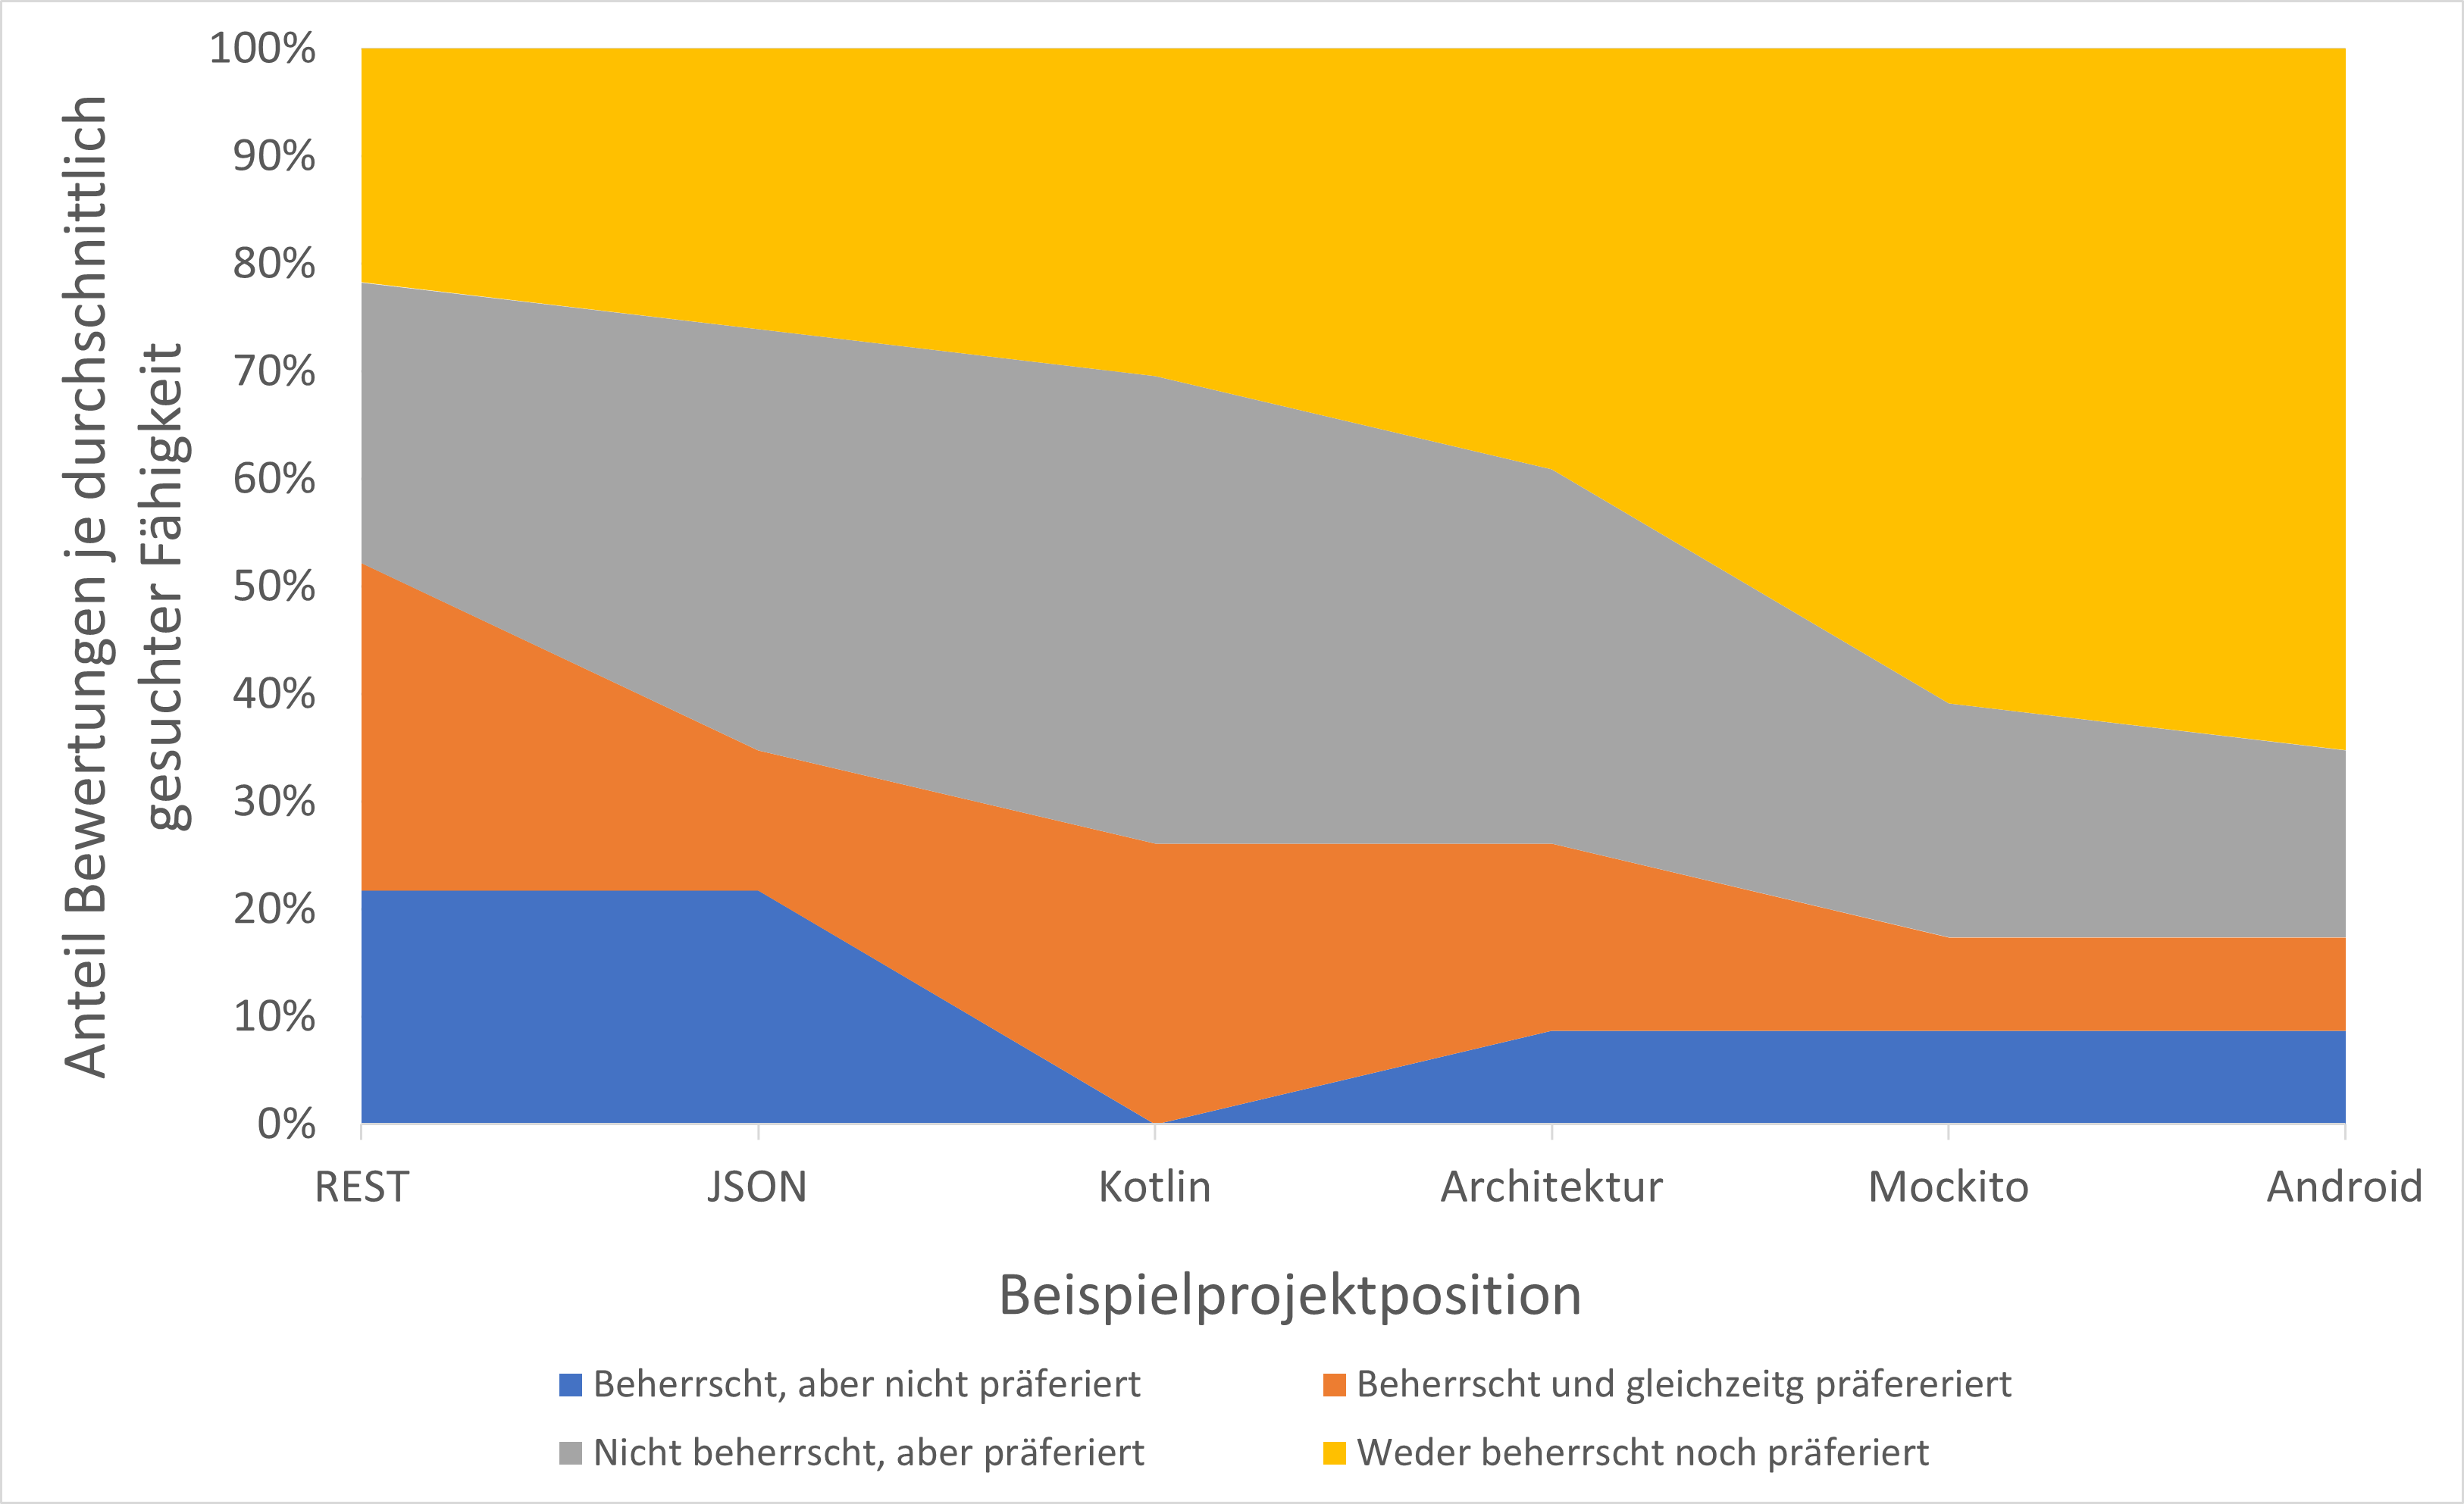
\includegraphics[width = 1\textwidth]{gfx/projekt-detail-e.png}}
	
	\caption{TODO Ansätze zur Berechnung des Vertrauens zwischen potentiellen Teammitgliedern \cite[S. 5]{malinowski:2005}}
	\label{fig:ergebnisse:analyse:abb6}
\end{figure}


\newpage

- Wie viel von gesuchten Fähigkeiten aus Projekten aus Long Tail?
- Wenn ich einen Mitarbeiter für eine bestimmte Technologie suche, wird er diese in 50 Prozent aller Fälle nicht präferieren

- Wie viele Cloud, KI? --> Wie viele nur 1 Bewertung (Ausreißer)
- Kein Coldstart bei Präferenzen
- Es sind immer mind. 19 andere Personen auf einem Skill verbunden

Projekt A: unilateral/bilateral\\
Projekt B: bilateral/unilateral\\
Projekt C: bilateral/unilateral\\
Projekt D: unilateral/bilateral\\
Projekt E: unilateral/bilateral

\shorthandon{"}
